\documentclass{article}

\usepackage{arxiv}

\usepackage[utf8]{inputenc} % allow utf-8 input
\usepackage[T1]{fontenc}    % use 8-bit T1 fonts
\usepackage{lmodern}        % https://github.com/rstudio/rticles/issues/343
\usepackage{hyperref}       % hyperlinks
\usepackage{url}            % simple URL typesetting
\usepackage{booktabs}       % professional-quality tables
\usepackage{amsfonts}       % blackboard math symbols
\usepackage{nicefrac}       % compact symbols for 1/2, etc.
\usepackage{microtype}      % microtypography
\usepackage{graphicx}

\title{Estimating Treatment Effects in Longitudinal Clinical Trials with
Missing Data}

\author{
    Amy Browne
   \\
    School of Mathematical and Statistical Sciences \\
    University of Galway \\
   \\
  \texttt{\href{mailto:a.browne47@universityofgalway.ie}{\nolinkurl{a.browne47@universityofgalway.ie}}} \\
   \And
    Tsz Mang Yip
   \\
    School of Mathematical and Statistical Sciences \\
    University of Galway \\
   \\
  \texttt{\href{mailto:k.yip2@universityofgalway.ie}{\nolinkurl{k.yip2@universityofgalway.ie}}} \\
  }

% Pandoc syntax highlighting
\usepackage{color}
\usepackage{fancyvrb}
\newcommand{\VerbBar}{|}
\newcommand{\VERB}{\Verb[commandchars=\\\{\}]}
\DefineVerbatimEnvironment{Highlighting}{Verbatim}{commandchars=\\\{\}}
% Add ',fontsize=\small' for more characters per line
\usepackage{framed}
\definecolor{shadecolor}{RGB}{248,248,248}
\newenvironment{Shaded}{\begin{snugshade}}{\end{snugshade}}
\newcommand{\AlertTok}[1]{\textcolor[rgb]{0.94,0.16,0.16}{#1}}
\newcommand{\AnnotationTok}[1]{\textcolor[rgb]{0.56,0.35,0.01}{\textbf{\textit{#1}}}}
\newcommand{\AttributeTok}[1]{\textcolor[rgb]{0.13,0.29,0.53}{#1}}
\newcommand{\BaseNTok}[1]{\textcolor[rgb]{0.00,0.00,0.81}{#1}}
\newcommand{\BuiltInTok}[1]{#1}
\newcommand{\CharTok}[1]{\textcolor[rgb]{0.31,0.60,0.02}{#1}}
\newcommand{\CommentTok}[1]{\textcolor[rgb]{0.56,0.35,0.01}{\textit{#1}}}
\newcommand{\CommentVarTok}[1]{\textcolor[rgb]{0.56,0.35,0.01}{\textbf{\textit{#1}}}}
\newcommand{\ConstantTok}[1]{\textcolor[rgb]{0.56,0.35,0.01}{#1}}
\newcommand{\ControlFlowTok}[1]{\textcolor[rgb]{0.13,0.29,0.53}{\textbf{#1}}}
\newcommand{\DataTypeTok}[1]{\textcolor[rgb]{0.13,0.29,0.53}{#1}}
\newcommand{\DecValTok}[1]{\textcolor[rgb]{0.00,0.00,0.81}{#1}}
\newcommand{\DocumentationTok}[1]{\textcolor[rgb]{0.56,0.35,0.01}{\textbf{\textit{#1}}}}
\newcommand{\ErrorTok}[1]{\textcolor[rgb]{0.64,0.00,0.00}{\textbf{#1}}}
\newcommand{\ExtensionTok}[1]{#1}
\newcommand{\FloatTok}[1]{\textcolor[rgb]{0.00,0.00,0.81}{#1}}
\newcommand{\FunctionTok}[1]{\textcolor[rgb]{0.13,0.29,0.53}{\textbf{#1}}}
\newcommand{\ImportTok}[1]{#1}
\newcommand{\InformationTok}[1]{\textcolor[rgb]{0.56,0.35,0.01}{\textbf{\textit{#1}}}}
\newcommand{\KeywordTok}[1]{\textcolor[rgb]{0.13,0.29,0.53}{\textbf{#1}}}
\newcommand{\NormalTok}[1]{#1}
\newcommand{\OperatorTok}[1]{\textcolor[rgb]{0.81,0.36,0.00}{\textbf{#1}}}
\newcommand{\OtherTok}[1]{\textcolor[rgb]{0.56,0.35,0.01}{#1}}
\newcommand{\PreprocessorTok}[1]{\textcolor[rgb]{0.56,0.35,0.01}{\textit{#1}}}
\newcommand{\RegionMarkerTok}[1]{#1}
\newcommand{\SpecialCharTok}[1]{\textcolor[rgb]{0.81,0.36,0.00}{\textbf{#1}}}
\newcommand{\SpecialStringTok}[1]{\textcolor[rgb]{0.31,0.60,0.02}{#1}}
\newcommand{\StringTok}[1]{\textcolor[rgb]{0.31,0.60,0.02}{#1}}
\newcommand{\VariableTok}[1]{\textcolor[rgb]{0.00,0.00,0.00}{#1}}
\newcommand{\VerbatimStringTok}[1]{\textcolor[rgb]{0.31,0.60,0.02}{#1}}
\newcommand{\WarningTok}[1]{\textcolor[rgb]{0.56,0.35,0.01}{\textbf{\textit{#1}}}}

% tightlist command for lists without linebreak
\providecommand{\tightlist}{%
  \setlength{\itemsep}{0pt}\setlength{\parskip}{0pt}}

% From pandoc table feature
\usepackage{longtable,booktabs,array}
\usepackage{calc} % for calculating minipage widths
% Correct order of tables after \paragraph or \subparagraph
\usepackage{etoolbox}
\makeatletter
\patchcmd\longtable{\par}{\if@noskipsec\mbox{}\fi\par}{}{}
\makeatother
% Allow footnotes in longtable head/foot
\IfFileExists{footnotehyper.sty}{\usepackage{footnotehyper}}{\usepackage{footnote}}
\makesavenoteenv{longtable}

% Pandoc citation processing
%From Pandoc 3.1.8
% definitions for citeproc citations
\NewDocumentCommand\citeproctext{}{}
\NewDocumentCommand\citeproc{mm}{%
  \begingroup\def\citeproctext{#2}\cite{#1}\endgroup}
\makeatletter
 % allow citations to break across lines
 \let\@cite@ofmt\@firstofone
 % avoid brackets around text for \cite:
 \def\@biblabel#1{}
 \def\@cite#1#2{{#1\if@tempswa , #2\fi}}
\makeatother
\newlength{\cslhangindent}
\setlength{\cslhangindent}{1.5em}
\newlength{\csllabelwidth}
\setlength{\csllabelwidth}{3em}
\newenvironment{CSLReferences}[2] % #1 hanging-indent, #2 entry-spacing
 {\begin{list}{}{%
  \setlength{\itemindent}{0pt}
  \setlength{\leftmargin}{0pt}
  \setlength{\parsep}{0pt}
  % turn on hanging indent if param 1 is 1
  \ifodd #1
   \setlength{\leftmargin}{\cslhangindent}
   \setlength{\itemindent}{-1\cslhangindent}
  \fi
  % set entry spacing
  \setlength{\itemsep}{#2\baselineskip}}}
 {\end{list}}
\usepackage{calc}
\newcommand{\CSLBlock}[1]{#1\hfill\break}
\newcommand{\CSLLeftMargin}[1]{\parbox[t]{\csllabelwidth}{#1}}
\newcommand{\CSLRightInline}[1]{\parbox[t]{\linewidth - \csllabelwidth}{#1}\break}
\newcommand{\CSLIndent}[1]{\hspace{\cslhangindent}#1}

\usepackage{amsmath}
\newcommand{\pandocbounded}[1]{#1}
\usepackage{float}
\floatplacement{figure}{H}
\usepackage{makecell}
\begin{document}
\maketitle


\begin{abstract}
\textbf{Motivation} Missing data is a pervasive issue in longitudinal
clinical trials, potentially introducing bias and reducing statistical
power. This project tested different missing data handling techniques,
using two real-world longitudinal randomized clinical trial (RCT)
datasets. \textbf{Results} No substantial differences were observed
between the methods across both datasets.
\textbf{Supplementary Information} Code is available at
\url{https://github.com/amydebrun/Missing-Data}.
\end{abstract}

\keywords{
    Missing Data
   \and
    Longitudinal Data
   \and
    Randomized Clinical Trial
   \and
    Real World Data Analysis
   \and
    Sensitivity Analysis
   \and
    Multiple Imputation
   \and
    Missingness Mechanisms
  }

\newpage

\section{Introduction}\label{introduction}

\subsection{Missing data in longitudinal
study}\label{missing-data-in-longitudinal-study}

\emph{Longitudinal Study Design}

Longitudinal studies are research designs in which data are collected
from the same participants at multiple time points. They provide
valuable insights into how variables change over time---often over
several years or decades. While this design is powerful for
understanding causal relationships and long-term trends, it presents
significant challenges in retaining participants across all waves of
data collection.

Longitudinal trials require consistent data collection methods at
predefined intervals. Researchers must work to minimize participant
dropout or non-response. However, due to the extended duration and
complexity of these studies, missing data is almost inevitable.

Similarly, clinical trials which evaluate the effects of biomedical or
behavioral interventions are also vulnerable to missing data.
Participants may miss follow-ups due to illness or other commitments.
This loss of data can compromise the study's validity. Ignoring missing
data introduces bias, as we're disregarding potentially informative
cases. For instance, if participants drop out due to adverse effects
from the treatment, the missing data is not random---this introduces
attrition bias, which can distort estimates of the treatment's effect.

Removing incomplete cases reduces the sample size, which in turn
decreases statistical power, limiting the ability to detect valid
treatment effects.

In statistical software like R, missing values are represented as NA
among the observed values. In longitudinal data, rows of data belonging
to individuals at a certain time-point can be missing. When fitting
models like linear regression, R automatically excludes any subjects
with missing values in either predictor or outcome variables. While
convenient, this method can lead to selection bias if the missingness is
systematic.

\subsection{Project Objective}\label{project-objective}

The objective of this project is to estimate treatment effects using
real-world data, with a primary focus on addressing issues that come
with missing data in clinical trials. We will briefly discuss different
assumptions about missing data mechanisms---such as Missing Completely
at Random, Missing at Random, and Missing Not at Random and investigate
their implications for statistical analysis.

While a range of methods are available to handle missing data, they all
vary in levels of complexity and assumptions. This project aims to
explore these methods, understand the reasons behind their differing
performance, and implement them on real-world longitudinal clinical data
to compare their ability to estimate treatment effect under real-world
conditions.

After initial exploration of the different methods, we also decided to
adjust the estimands through data wrangling our chosen datasets to
compare how the estimate differs when the estimand is either categorical
or continuous and to compare the effects using linear regression or
linear mixed effects models. Additionally, we will conduct sensitivity
analyses to investigate how treatment effect estimates change under
different assumptions about the missing data.

\subsection{Missingness Mechanisms}\label{missingness-mechanisms}

Missing data mechanisms are important to consider when choosing which
sort of missing data handling method to use. There are three mechanisms
which missing data can follow:

\begin{itemize}
\tightlist
\item
  Missing Completely At Random (MCAR)
\item
  Missing At Random (MAR)
\item
  Missing Not At Random (MNAR)
\end{itemize}

Although they may appear similar at first glance, continuing to handle
missing data without considering these mechanisms may still result in
biased estimates and inaccurate conclusions. Missing data mechanisms
appear to be mentioned first by Donald Rubin in 1976. We can formally
define these mechanisms using the following notation;

\begin{itemize}
\tightlist
\item
  \(R\) represents a missing data indicator which when \(R=1\) indicates
  observed data and \(R=0\) indicates unobserved
\item
  \(X\) represents data that is always observed
\item
  \(Y\) represents data that is potentially missing.
\end{itemize}

\textbf{Missing Completely At Random}

The formal definition of MCAR data is:

\[\quad P(R = 1 \mid Y, X) = P(R = 1)\] The probability of the data is
observed given observed data and missing data is the same as the
probability of being observed without the given data. This mechanism is
considered the easiest to deal with as it does not bias the result
although data is rarely MCAR. This can occur due to system failure and
some data is deleted accidentally, or else there is issues with the
treatment system and data cannot be recorded. The DAG below visualises
an example of this mechanism based on a randomised trial with
randomisation variable \(L\). Missing indicator \(R_Y\), which denotes
whether the outcome is observed (\(R_Y = 1\)) or missing (\(R_Y = 0\)),
is independent from the observed baseline variables \(X_1\) and \(X_2\),
which are pre-randomised variables, and outcome variable \(Y\) (which
potentially contains missing data).

\begin{figure}
\centering
\pandocbounded{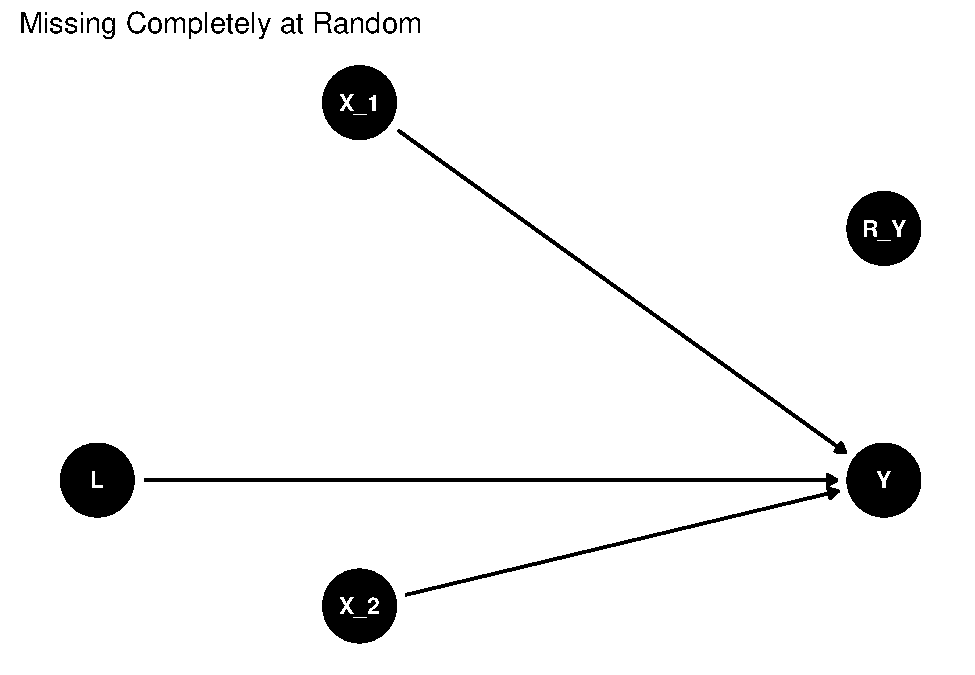
\includegraphics[keepaspectratio]{Final_Report_files/figure-latex/unnamed-chunk-1-1.pdf}}
\caption{MCAR DAG}
\end{figure}

\textbf{Missing At Random}

\[\quad P(R = 1 \mid Y, X) = P(R = 1 \mid X)\] The probability of data
being observed given observed and unobserved data is the same as the
probability being observed given the observed data. In short, the
missing data dependends on the observed data. We can say that the
missing data indicator is conditional on another variable.

MAR is a more realistic mechanism than MCAR and requires more intensive
handling methods. Below shows 2 DAGs that shows a general example of a
randomised treatment \(L\) on response variable \(Y\), which potentially
contains missing data. \(X_1\) and \(X_2\) are baseline variables,
recorded pre-randomisation. The first DAG shows the MAR mechanism
conditioned on both baseline variables; missingness indicator \(R_Y\) is
influenced by baseline variables \(X_1\) and \(X_2\). The second DAG is
similar, but shows the data is MAR conditional on randomised treatment
\(L\) and baseline variable \(X_1\). \(X_2\) no longer influences the
missingness indicator \(R_Y\), but \(R_Y\) is still conditioned on \(L\)
and \(X_1\), showing the MAR assumption still holds given these
variables.

\begin{figure}
\centering
\pandocbounded{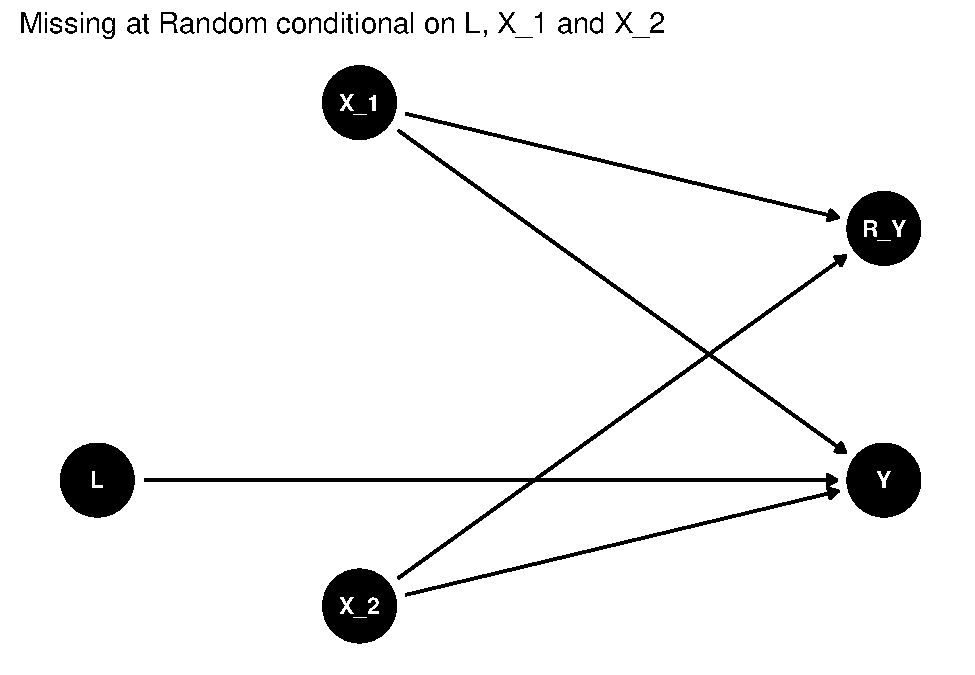
\includegraphics[keepaspectratio]{Final_Report_files/figure-latex/unnamed-chunk-2-1.pdf}}
\caption{Missing at Random conditional on L, X\_1 and X\_2}
\end{figure}

\begin{figure}
\centering
\pandocbounded{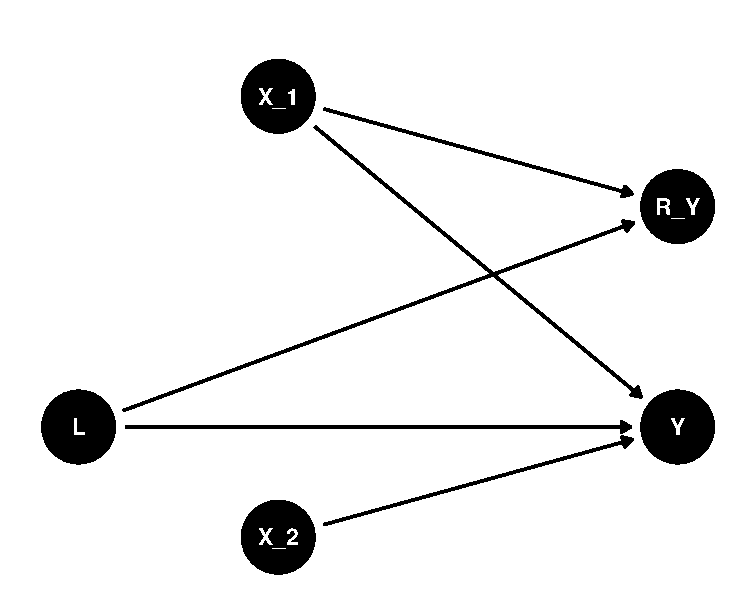
\includegraphics[keepaspectratio]{Final_Report_files/figure-latex/unnamed-chunk-3-1.pdf}}
\caption{Missing at Random conditional on L, X\_1}
\end{figure}

\textbf{Missing Not At Random}

\(\quad P(R = 1 \mid Y, X) \ne P(R = 1 \mid X)\) The probability of data
being observed depends both on the observed data and the missing data.
This mechanism is the most difficult to deal with as it relates to the
unobserved data, so producing valid results is a challenge. Certain
participants in a general health study may avoid answering questions
truthfully about smoking habits or their diet in order to make
themselves more appealing. Sensitivity analysis is an option to
determine the treatment effect when assuming different mechanisms. The 2
following DAGs show this mechanism using the above scenarios. In the
first DAGs structure, the potentially missing outcome variable \(Y\)
directly influences \(R_Y\). The outcome \(Y\) is directly influenced by
the randomised treatment \(L\) and baseline variables \(X_1\) and
\(X_2\), but the missingness indicator is influenced by the missing
outcome data. The second DAG shows MNAR conditional on \(X_2\) only as
it influences the missingness indicator \(R_Y\) along with the missing
outcome.

\begin{figure}
\centering
\pandocbounded{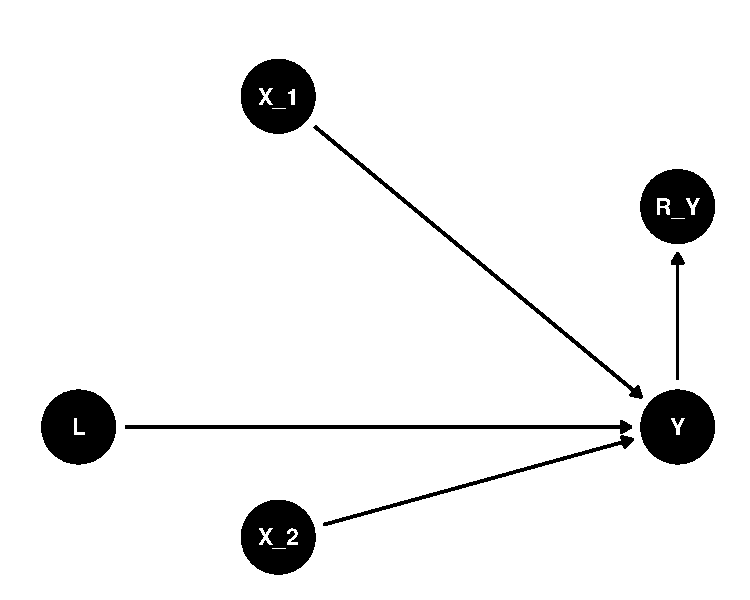
\includegraphics[keepaspectratio]{Final_Report_files/figure-latex/unnamed-chunk-4-1.pdf}}
\caption{Missing not at Random conditional on L, X\_1 and X\_2}
\end{figure}

\begin{figure}
\centering
\pandocbounded{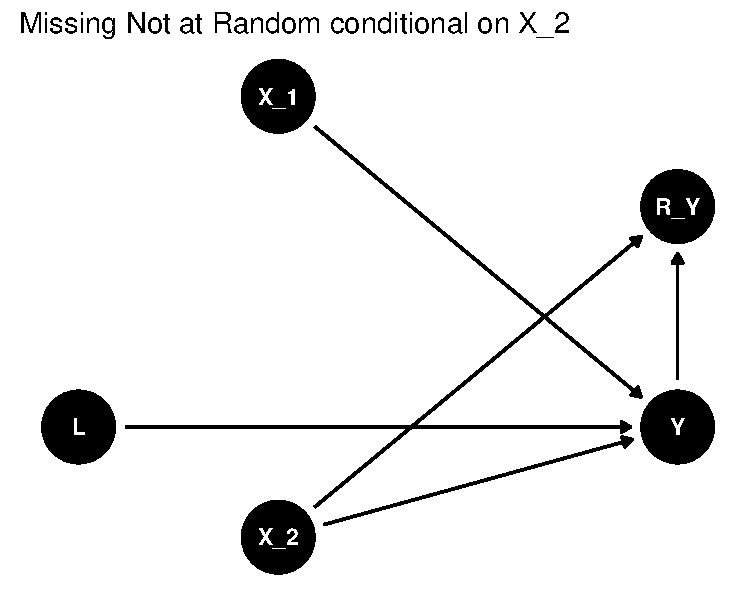
\includegraphics[keepaspectratio]{Final_Report_files/figure-latex/unnamed-chunk-5-1.pdf}}
\caption{Missing at Random conditional on L, X\_2}
\end{figure}

Although these considerations are important, the mechanism underlying
missing data is fundamentally untestable. Since the true values of
missing observations are never observed, we cannot definitively
determine which missingness assumption holds in practice. There is
limited hypothesis test available to see whether data is MCAR
(\emph{Little's MCAR test}). It is a likelihood-ratio test that groups
missing data patterns, estimates the expected means under a multivariate
normal model using maximum likelihood, and computes a chi-square
statistic to assess model fit. The decision lies under the hypotheses;

\begin{itemize}
\tightlist
\item
  \(H_0\): Data is MCAR
\item
  \(H_1\): Data is MAR or MNAR
\end{itemize}

If the p-value resulting from the chi-square distribution is greater
than 0.05, we fail to reject the null hypothesis. It is limited as it
does not necessarily confirm MCAR but provides no evidence to reject
that the data MCAR. If the test has a significant p-value, it suggests
that the data is either MAR or MNAR, but its unclear which one. This
test is also vulnerable to Type 1 error (false positive result) and Type
2 error (false negative result) as the test may not detect MCAR
violations with its low statistical power, even if the MCAR assumption
holds.

\subsection{Different missing data
patterns}\label{different-missing-data-patterns}

A missing data pattern describes the pattern of missing data among the
observed data. As described by Little \& Rubin (2014), it's important to
remark the missing data patterns of the data set prior to data handling
as some handling methods are intended for certain classified patterns.
The following table summarises some missing data patterns.

\begin{table}[H]
\centering
\caption{Missing Data Pattern}
\label{}

\begin{tabular}{ll}
\toprule
Pattern & Description\\
\midrule
Univariate & Missing values in a single variable\\
Multivariate & Missing values present in multiple variables\\
Monotonic & Variables $Y_j$ can be ordered such that if $Y_j$ is missing, all subsequent variables are also missing\\
General & Missing values have no structure and are scattered throughout data\\
\bottomrule
\end{tabular}
\end{table}

\subsection{Literature}\label{literature}

While reviewing the literature on missing data, it became evident that
despite the use of established handling methods, there remains room for
improvement in how missing data are addressed in clinical study reports
and in the selection of appropriate methods.

In 2014, Powney et al.~reviewed 100 longitudinal clinical trials
conducted between 2005 and 2012 and found that only 44 reported an
adequate method to handle missing data, while 30 used potentially
inadequate methods.

Spineli et al.~(2015) examined 190 systematic reviews published after
2009 to investigate how missing data were reported in randomized
controlled trials. Although 175 of these reviews mentioned missing data,
only 61 discussed its implications.

Hunt et al.~(2021) reviewed 62 pharmacoepidemiologic multi-database
studies from 2018 to 2019 to assess missing data reporting and handling.
Thirty-five studies reported missing data, but only 19 described methods
for handling it. The most popular approach was complete case analysis
(CCA) used in 13 studies, followed by multiple imputation (MI) in 2
studies.

Complete case analysis was also the predominant method in a systematic
review of 229 observational studies from the United Network for Organ
Sharing (UNOS) database (Baker et al., 2025). Forty-one studies used
CCA, 22 reported MI, and notably, 31 studies removed covariates due to
missing values---an action that could introduce further bias depending
on the covariates' relationship with other predictors.

\newpage

\section{Clinical Trial Data}\label{clinical-trial-data}

We have sourced two different data sets to perform our missingness
analysis on. They both have different sample sizes and different levels
of missing data which is an advantage as we can conduct analysis in
different settings.

\subsection{Acupuncture Data}\label{acupuncture-data}

Our first dataset contains results from a clinical trial determining the
effects of acupuncture therapy on chronic headache in primary care
(Vickers et al 2004). Vickers released the dataset from the study in
2006 and is publicly available to download in excel format from
\url{https://pmc.ncbi.nlm.nih.gov/articles/PMC1489946/}. The study
design for the acupuncture trial is a longitudinal randomised controlled
trial with two follow up time points. 401 participants were gathered
from general practices in England and Wales who suffered from migraines.
The main objective was to determine the effects of acupuncture use on
headache severity, health status, absence days and GP and therapist
visits in comparison to avoiding acupuncture against a control
intervention whih offered standard care. Headache and medication use was
recorded at baseline and additional factors were recorded
post-randomisation such as such sick days and daily activities. The
results of the trial showed a 34\% decrease in headache severity score
at the final time point in comparison to the control group with a 16\%
decrease. The acupuncture therapy group also showed a 37\% decrease in
medication use, which compares to 23\% in the control group.

\subsubsection{Data Overview}\label{data-overview}

13 variables were recorded during the acupuncture trial.

\begin{table}[H]
\centering
\caption{Acupuncture trial variables}
\label{}

\begin{tabular}{ll}
\toprule
Variable & Description\\
\midrule
id & patient ID code\\
age & Age\\
sex & sex; female (1) vs. male (0)\\
migraine & diagnosis ; migraine (1) vs. tension-type (0)\\
chronicity & number of years of headache disorder\\
\addlinespace
acupuncturist & acupuncturist id code\\
practiceid & gp practice id\\
group & treatment group; acupuncture (1) vs. control (0)\\
pk1 & headache severity score baseline\\
pk2 & headache severity score 3 month\\
\addlinespace
pk5 & headache severity score 1 year\\
f1 & headache frequency baseline\\
f2 & headache frequency 3 month\\
f5 & headache frequency 1 year\\
\bottomrule
\end{tabular}
\end{table}

Variables \texttt{pk2} and \texttt{pk5} are the headache severity scores
at 3 months and 12 months.

\begin{table}

\caption{Acupuncture data overview}
\centering
\begin{tabular}[t]{l|c|c}
\hline
\textbf{Characteristic} & \makecell[c]{\textbf{0}\ \ \\N = 196} & \makecell[c]{\textbf{1}\ \ \\N = 205}\\
\hline
id & 470 (209) & 472 (206)\\
\hline
age & 45 (11) & 46 (11)\\
\hline
sex & 165(84\%) & 172(84\%)\\
\hline
migraine & 183(93\%) & 194(95\%)\\
\hline
chronicity & 22 (13) & 21 (14)\\
\hline
acupuncturist & 5.97 (2.82) & 6.00 (2.80)\\
\hline
practice\_id & 24 (11) & 25 (12)\\
\hline
pk1 & 27 (17) & 26 (15)\\
\hline
pk2 & 24 (18) & 19 (16)\\
\hline
\hspace{1em}Missing & 43 & 32\\
\hline
pk5 & 22 (17) & 16 (14)\\
\hline
\hspace{1em}Missing & 56 & 44\\
\hline
f1 & 16 (7) & 16 (7)\\
\hline
f2 & 11 (9) & 11 (8)\\
\hline
f5 & 10 (9) & 9 (8)\\
\hline
\multicolumn{3}{l}{\rule{0pt}{1em}\textsuperscript{1} Mean (SD); n(\%)}\\
\end{tabular}
\end{table}

Table 2.x are the summary statistics of the acupuncture trial data.
These consist of 2 columns; column 0 showing control group statistics
and column 1 showing treatment group statistics. The continous variables
show the mean value (standard deviation) and the categorical variables
show the count(percentage). Note pk2 and pk5 are post randomisation
variables and contain missing data.

\begin{figure}
\centering
\pandocbounded{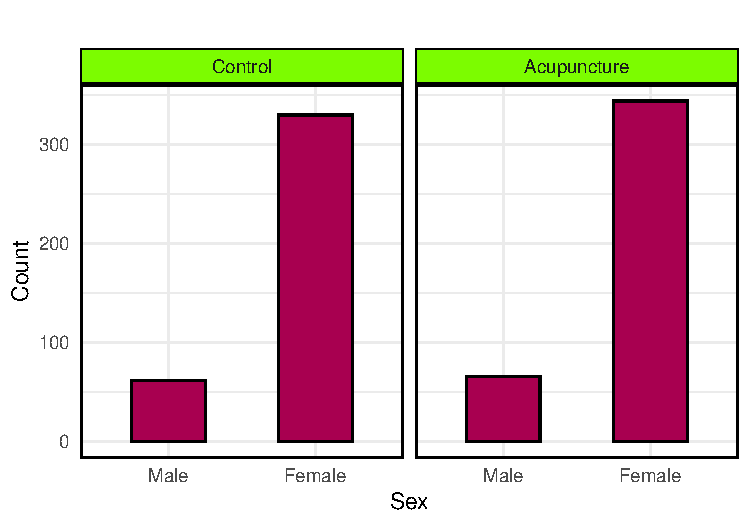
\includegraphics[keepaspectratio]{Final_Report_files/figure-latex/unnamed-chunk-9-1.pdf}}
\caption{The distribution of sex in both treatment groups of the
acupuncture trial data. The participants are predominantly female.}
\end{figure}

\begin{figure}
\centering
\pandocbounded{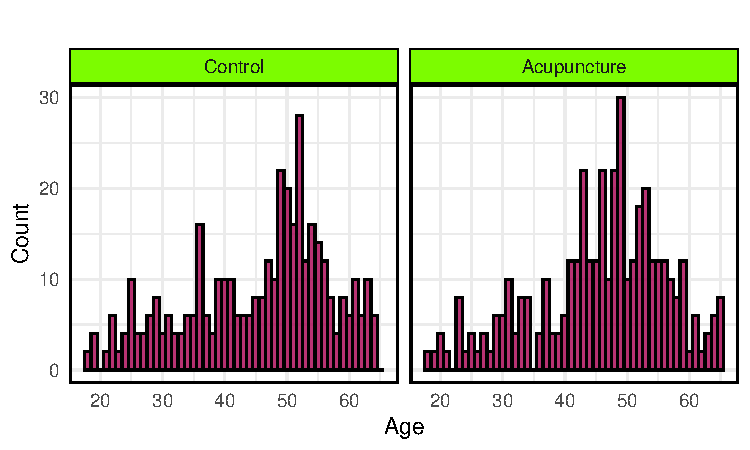
\includegraphics[keepaspectratio]{Final_Report_files/figure-latex/unnamed-chunk-10-1.pdf}}
\caption{The distribution of age in both treatment groups. Both
distributions are negatively skewed, predominantly middle aged and
older.}
\end{figure}

\pandocbounded{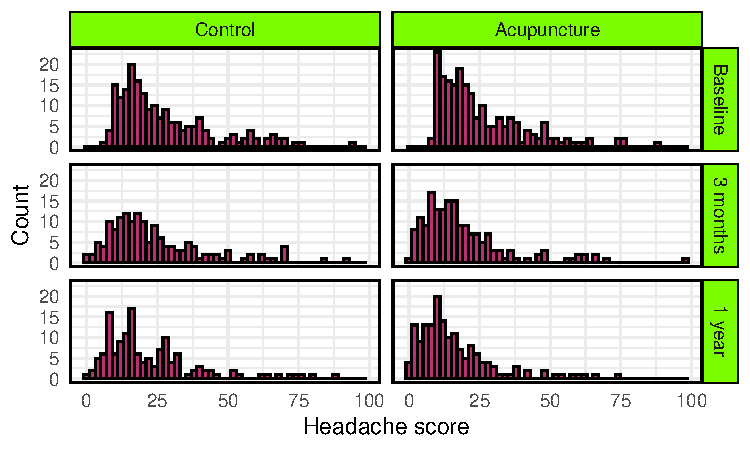
\includegraphics[keepaspectratio]{Final_Report_files/figure-latex/unnamed-chunk-11-1.pdf}}

\pandocbounded{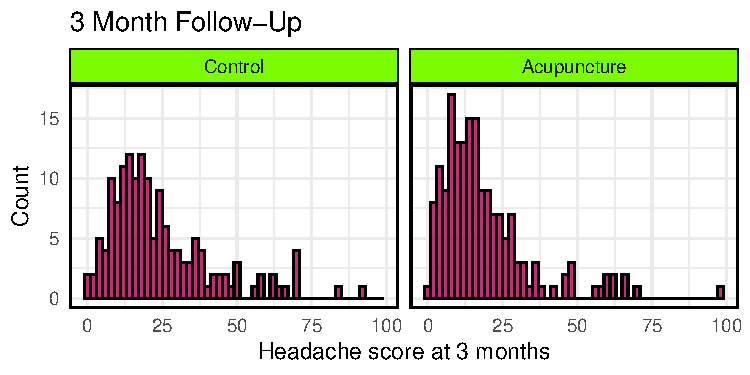
\includegraphics[keepaspectratio]{Final_Report_files/figure-latex/unnamed-chunk-12-1.pdf}}

\pandocbounded{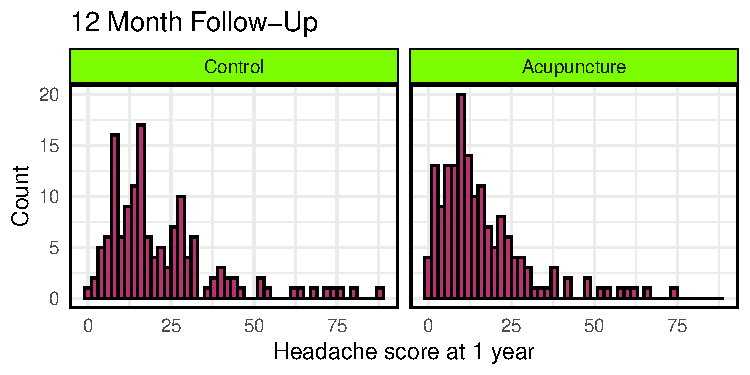
\includegraphics[keepaspectratio]{Final_Report_files/figure-latex/unnamed-chunk-13-1.pdf}}

Figure 2.x,2.x,2.x: These plots show the distribution of the headache
severity score at the three measured time-points. Over the three
time-points we can see a generally positively skewed distribution with
most headache severity scores ranging between 0 and 35. There appears to
be minimal difference in headache severity score over the treatment
group, and the control group appears to have a lower headache severity
score overall. The 3 month and 12 month time-point distributions are
incomplete due to the missing values.

\subsection{VITAL data}\label{vital-data}

The Vitamin D and Omega-3 trial (VITAL) was a nationwide clinical trial
to determine the effects of daily doses of 2000 IU vitamin D and 1 gram
of omega-3 fatty acids (fishoil) on preventing cancer and cardiovascular
disease (CVD). This was a 2x2 factorial designed longitudinal randomised
controlled trial in which 25,871 adults were randomised to 4 possible
combinations of treatment; fish oil, vitamin D, both treatments, an a
control group with no treatment. The results of the vitamin D group said
that it did not lower cancer development significantly neither did it
cause any meaningful reuction in cardiovascular disease. As for the
fish-oil intervention lowered risk of heart attack by 28\% and risk of
heart attack fatality by 50\%, but no reduction in stroke or non-heart
disease cardiovascular fatalities. Fish oil did not reduce occurence in
breast or prostate cancer or cancer-deaths. For our research, we are
analysing the results of an ancillary study which uses data from VITAL.
MacFarlane et al (2020) conducted a study using VITAL on the therapeutic
effects of vitamin D and fishoil on osteoarthritic knee pain. 1,398
participants in the study was randomised to 4 possible treatment
combinations. Participants were randomised to receive either omega-3
oils or vitamin D, both treatments, or randomised to the placebo group.
A knee pain scale grading index Western Ontario and McMaster
Osteoarthritis Index (WOMAC) is used to record knee pain score at
baseline and annually for 4 time-points post randomisation. Results
showed that there was no significant change in knee pain score between
both treatment groups and the control group. For this research project,
we assumed that that the participants were only randomised to either
receive the fish oil treatment, vitamin D treatment or the placebo. We
did not include the interaction between vitamin D and fish oil in our
models. The below table shows the sample size per treatment group.

\begin{longtable}[]{@{}lll@{}}
\toprule\noalign{}
& \textbf{Vitamin D} & \textbf{Placebo} \\
\midrule\noalign{}
\endhead
\bottomrule\noalign{}
\endlastfoot
\textbf{Fish Oil} & N = 342 \emph{(not analysed)} & N = 353 \\
\textbf{Placebo} & N = 332 & N = 371 \\
\end{longtable}

\subsubsection{Data Overview}\label{data-overview-1}

There are x variables recorded in the VITAL data, the following table
refers to a subset of the variables that we frequently use.

\begin{verbatim}
## \begin{table}[H]
## \centering
## \caption{VITAL study variables}
## \label{}
\end{verbatim}

\begin{verbatim}
## 
## \begin{tabular}{ll}
## \toprule
## Variable & Description\\
## \midrule
## Subject_ID & Patient ID code\\
## age & Age of patient\\
## bmi & Body mass index of patient\\
## sex & Sex of patient\\
## vitdactive & 1=vitamin D, 0=no vitamin D\\
## \addlinespace
## fishoilactive & 1= fish oil, 0= no fish oil\\
## pain_base & Knee pain at baseline\\
## pain_yrX & Knee pain X years post randomisation\\
## stiffness_base & Knee stiffness at baseline\\
## stiffness_yrX & Knee stiffness X years post randomisation\\
## \addlinespace
## function_base & Knee function at baseline\\
## function_yrX & Knee function X years post randomisation\\
## kneepainfreq & Frequency of knee pain\\
## \bottomrule
## \end{tabular}
\end{verbatim}

\begin{verbatim}
## \end{table}
\end{verbatim}

\begin{verbatim}
## <div id="fusrtpmjgp" style="padding-left:0px;padding-right:0px;padding-top:10px;padding-bottom:10px;overflow-x:auto;overflow-y:auto;width:auto;height:auto;">
##   <style>#fusrtpmjgp table {
##   font-family: system-ui, 'Segoe UI', Roboto, Helvetica, Arial, sans-serif, 'Apple Color Emoji', 'Segoe UI Emoji', 'Segoe UI Symbol', 'Noto Color Emoji';
##   -webkit-font-smoothing: antialiased;
##   -moz-osx-font-smoothing: grayscale;
## }
## 
## #fusrtpmjgp thead, #fusrtpmjgp tbody, #fusrtpmjgp tfoot, #fusrtpmjgp tr, #fusrtpmjgp td, #fusrtpmjgp th {
##   border-style: none;
## }
## 
## #fusrtpmjgp p {
##   margin: 0;
##   padding: 0;
## }
## 
## #fusrtpmjgp .gt_table {
##   display: table;
##   border-collapse: collapse;
##   line-height: normal;
##   margin-left: auto;
##   margin-right: auto;
##   color: #333333;
##   font-size: 16px;
##   font-weight: normal;
##   font-style: normal;
##   background-color: #FFFFFF;
##   width: auto;
##   border-top-style: solid;
##   border-top-width: 2px;
##   border-top-color: #A8A8A8;
##   border-right-style: none;
##   border-right-width: 2px;
##   border-right-color: #D3D3D3;
##   border-bottom-style: solid;
##   border-bottom-width: 2px;
##   border-bottom-color: #A8A8A8;
##   border-left-style: none;
##   border-left-width: 2px;
##   border-left-color: #D3D3D3;
## }
## 
## #fusrtpmjgp .gt_caption {
##   padding-top: 4px;
##   padding-bottom: 4px;
## }
## 
## #fusrtpmjgp .gt_title {
##   color: #333333;
##   font-size: 125%;
##   font-weight: initial;
##   padding-top: 4px;
##   padding-bottom: 4px;
##   padding-left: 5px;
##   padding-right: 5px;
##   border-bottom-color: #FFFFFF;
##   border-bottom-width: 0;
## }
## 
## #fusrtpmjgp .gt_subtitle {
##   color: #333333;
##   font-size: 85%;
##   font-weight: initial;
##   padding-top: 3px;
##   padding-bottom: 5px;
##   padding-left: 5px;
##   padding-right: 5px;
##   border-top-color: #FFFFFF;
##   border-top-width: 0;
## }
## 
## #fusrtpmjgp .gt_heading {
##   background-color: #FFFFFF;
##   text-align: center;
##   border-bottom-color: #FFFFFF;
##   border-left-style: none;
##   border-left-width: 1px;
##   border-left-color: #D3D3D3;
##   border-right-style: none;
##   border-right-width: 1px;
##   border-right-color: #D3D3D3;
## }
## 
## #fusrtpmjgp .gt_bottom_border {
##   border-bottom-style: solid;
##   border-bottom-width: 2px;
##   border-bottom-color: #D3D3D3;
## }
## 
## #fusrtpmjgp .gt_col_headings {
##   border-top-style: solid;
##   border-top-width: 2px;
##   border-top-color: #D3D3D3;
##   border-bottom-style: solid;
##   border-bottom-width: 2px;
##   border-bottom-color: #D3D3D3;
##   border-left-style: none;
##   border-left-width: 1px;
##   border-left-color: #D3D3D3;
##   border-right-style: none;
##   border-right-width: 1px;
##   border-right-color: #D3D3D3;
## }
## 
## #fusrtpmjgp .gt_col_heading {
##   color: #333333;
##   background-color: #FFFFFF;
##   font-size: 100%;
##   font-weight: normal;
##   text-transform: inherit;
##   border-left-style: none;
##   border-left-width: 1px;
##   border-left-color: #D3D3D3;
##   border-right-style: none;
##   border-right-width: 1px;
##   border-right-color: #D3D3D3;
##   vertical-align: bottom;
##   padding-top: 5px;
##   padding-bottom: 6px;
##   padding-left: 5px;
##   padding-right: 5px;
##   overflow-x: hidden;
## }
## 
## #fusrtpmjgp .gt_column_spanner_outer {
##   color: #333333;
##   background-color: #FFFFFF;
##   font-size: 100%;
##   font-weight: normal;
##   text-transform: inherit;
##   padding-top: 0;
##   padding-bottom: 0;
##   padding-left: 4px;
##   padding-right: 4px;
## }
## 
## #fusrtpmjgp .gt_column_spanner_outer:first-child {
##   padding-left: 0;
## }
## 
## #fusrtpmjgp .gt_column_spanner_outer:last-child {
##   padding-right: 0;
## }
## 
## #fusrtpmjgp .gt_column_spanner {
##   border-bottom-style: solid;
##   border-bottom-width: 2px;
##   border-bottom-color: #D3D3D3;
##   vertical-align: bottom;
##   padding-top: 5px;
##   padding-bottom: 5px;
##   overflow-x: hidden;
##   display: inline-block;
##   width: 100%;
## }
## 
## #fusrtpmjgp .gt_spanner_row {
##   border-bottom-style: hidden;
## }
## 
## #fusrtpmjgp .gt_group_heading {
##   padding-top: 8px;
##   padding-bottom: 8px;
##   padding-left: 5px;
##   padding-right: 5px;
##   color: #333333;
##   background-color: #FFFFFF;
##   font-size: 100%;
##   font-weight: initial;
##   text-transform: inherit;
##   border-top-style: solid;
##   border-top-width: 2px;
##   border-top-color: #D3D3D3;
##   border-bottom-style: solid;
##   border-bottom-width: 2px;
##   border-bottom-color: #D3D3D3;
##   border-left-style: none;
##   border-left-width: 1px;
##   border-left-color: #D3D3D3;
##   border-right-style: none;
##   border-right-width: 1px;
##   border-right-color: #D3D3D3;
##   vertical-align: middle;
##   text-align: left;
## }
## 
## #fusrtpmjgp .gt_empty_group_heading {
##   padding: 0.5px;
##   color: #333333;
##   background-color: #FFFFFF;
##   font-size: 100%;
##   font-weight: initial;
##   border-top-style: solid;
##   border-top-width: 2px;
##   border-top-color: #D3D3D3;
##   border-bottom-style: solid;
##   border-bottom-width: 2px;
##   border-bottom-color: #D3D3D3;
##   vertical-align: middle;
## }
## 
## #fusrtpmjgp .gt_from_md > :first-child {
##   margin-top: 0;
## }
## 
## #fusrtpmjgp .gt_from_md > :last-child {
##   margin-bottom: 0;
## }
## 
## #fusrtpmjgp .gt_row {
##   padding-top: 8px;
##   padding-bottom: 8px;
##   padding-left: 5px;
##   padding-right: 5px;
##   margin: 10px;
##   border-top-style: solid;
##   border-top-width: 1px;
##   border-top-color: #D3D3D3;
##   border-left-style: none;
##   border-left-width: 1px;
##   border-left-color: #D3D3D3;
##   border-right-style: none;
##   border-right-width: 1px;
##   border-right-color: #D3D3D3;
##   vertical-align: middle;
##   overflow-x: hidden;
## }
## 
## #fusrtpmjgp .gt_stub {
##   color: #333333;
##   background-color: #FFFFFF;
##   font-size: 100%;
##   font-weight: initial;
##   text-transform: inherit;
##   border-right-style: solid;
##   border-right-width: 2px;
##   border-right-color: #D3D3D3;
##   padding-left: 5px;
##   padding-right: 5px;
## }
## 
## #fusrtpmjgp .gt_stub_row_group {
##   color: #333333;
##   background-color: #FFFFFF;
##   font-size: 100%;
##   font-weight: initial;
##   text-transform: inherit;
##   border-right-style: solid;
##   border-right-width: 2px;
##   border-right-color: #D3D3D3;
##   padding-left: 5px;
##   padding-right: 5px;
##   vertical-align: top;
## }
## 
## #fusrtpmjgp .gt_row_group_first td {
##   border-top-width: 2px;
## }
## 
## #fusrtpmjgp .gt_row_group_first th {
##   border-top-width: 2px;
## }
## 
## #fusrtpmjgp .gt_summary_row {
##   color: #333333;
##   background-color: #FFFFFF;
##   text-transform: inherit;
##   padding-top: 8px;
##   padding-bottom: 8px;
##   padding-left: 5px;
##   padding-right: 5px;
## }
## 
## #fusrtpmjgp .gt_first_summary_row {
##   border-top-style: solid;
##   border-top-color: #D3D3D3;
## }
## 
## #fusrtpmjgp .gt_first_summary_row.thick {
##   border-top-width: 2px;
## }
## 
## #fusrtpmjgp .gt_last_summary_row {
##   padding-top: 8px;
##   padding-bottom: 8px;
##   padding-left: 5px;
##   padding-right: 5px;
##   border-bottom-style: solid;
##   border-bottom-width: 2px;
##   border-bottom-color: #D3D3D3;
## }
## 
## #fusrtpmjgp .gt_grand_summary_row {
##   color: #333333;
##   background-color: #FFFFFF;
##   text-transform: inherit;
##   padding-top: 8px;
##   padding-bottom: 8px;
##   padding-left: 5px;
##   padding-right: 5px;
## }
## 
## #fusrtpmjgp .gt_first_grand_summary_row {
##   padding-top: 8px;
##   padding-bottom: 8px;
##   padding-left: 5px;
##   padding-right: 5px;
##   border-top-style: double;
##   border-top-width: 6px;
##   border-top-color: #D3D3D3;
## }
## 
## #fusrtpmjgp .gt_last_grand_summary_row_top {
##   padding-top: 8px;
##   padding-bottom: 8px;
##   padding-left: 5px;
##   padding-right: 5px;
##   border-bottom-style: double;
##   border-bottom-width: 6px;
##   border-bottom-color: #D3D3D3;
## }
## 
## #fusrtpmjgp .gt_striped {
##   background-color: rgba(128, 128, 128, 0.05);
## }
## 
## #fusrtpmjgp .gt_table_body {
##   border-top-style: solid;
##   border-top-width: 2px;
##   border-top-color: #D3D3D3;
##   border-bottom-style: solid;
##   border-bottom-width: 2px;
##   border-bottom-color: #D3D3D3;
## }
## 
## #fusrtpmjgp .gt_footnotes {
##   color: #333333;
##   background-color: #FFFFFF;
##   border-bottom-style: none;
##   border-bottom-width: 2px;
##   border-bottom-color: #D3D3D3;
##   border-left-style: none;
##   border-left-width: 2px;
##   border-left-color: #D3D3D3;
##   border-right-style: none;
##   border-right-width: 2px;
##   border-right-color: #D3D3D3;
## }
## 
## #fusrtpmjgp .gt_footnote {
##   margin: 0px;
##   font-size: 90%;
##   padding-top: 4px;
##   padding-bottom: 4px;
##   padding-left: 5px;
##   padding-right: 5px;
## }
## 
## #fusrtpmjgp .gt_sourcenotes {
##   color: #333333;
##   background-color: #FFFFFF;
##   border-bottom-style: none;
##   border-bottom-width: 2px;
##   border-bottom-color: #D3D3D3;
##   border-left-style: none;
##   border-left-width: 2px;
##   border-left-color: #D3D3D3;
##   border-right-style: none;
##   border-right-width: 2px;
##   border-right-color: #D3D3D3;
## }
## 
## #fusrtpmjgp .gt_sourcenote {
##   font-size: 90%;
##   padding-top: 4px;
##   padding-bottom: 4px;
##   padding-left: 5px;
##   padding-right: 5px;
## }
## 
## #fusrtpmjgp .gt_left {
##   text-align: left;
## }
## 
## #fusrtpmjgp .gt_center {
##   text-align: center;
## }
## 
## #fusrtpmjgp .gt_right {
##   text-align: right;
##   font-variant-numeric: tabular-nums;
## }
## 
## #fusrtpmjgp .gt_font_normal {
##   font-weight: normal;
## }
## 
## #fusrtpmjgp .gt_font_bold {
##   font-weight: bold;
## }
## 
## #fusrtpmjgp .gt_font_italic {
##   font-style: italic;
## }
## 
## #fusrtpmjgp .gt_super {
##   font-size: 65%;
## }
## 
## #fusrtpmjgp .gt_footnote_marks {
##   font-size: 75%;
##   vertical-align: 0.4em;
##   position: initial;
## }
## 
## #fusrtpmjgp .gt_asterisk {
##   font-size: 100%;
##   vertical-align: 0;
## }
## 
## #fusrtpmjgp .gt_indent_1 {
##   text-indent: 5px;
## }
## 
## #fusrtpmjgp .gt_indent_2 {
##   text-indent: 10px;
## }
## 
## #fusrtpmjgp .gt_indent_3 {
##   text-indent: 15px;
## }
## 
## #fusrtpmjgp .gt_indent_4 {
##   text-indent: 20px;
## }
## 
## #fusrtpmjgp .gt_indent_5 {
##   text-indent: 25px;
## }
## 
## #fusrtpmjgp .katex-display {
##   display: inline-flex !important;
##   margin-bottom: 0.75em !important;
## }
## 
## #fusrtpmjgp div.Reactable > div.rt-table > div.rt-thead > div.rt-tr.rt-tr-group-header > div.rt-th-group:after {
##   height: 0px !important;
## }
## </style>
##   <table class="gt_table" data-quarto-disable-processing="false" data-quarto-bootstrap="false">
##   <thead>
##     <tr class="gt_col_headings">
##       <th class="gt_col_heading gt_columns_bottom_border gt_left" rowspan="1" colspan="1" scope="col" id="label"><span class='gt_from_md'><strong>Characteristic</strong></span></th>
##       <th class="gt_col_heading gt_columns_bottom_border gt_center" rowspan="1" colspan="1" scope="col" id="stat_1"><span class='gt_from_md'><strong>Both</strong>  N = 342</span><span class="gt_footnote_marks" style="white-space:nowrap;font-style:italic;font-weight:normal;line-height:0;"><sup>1</sup></span></th>
##       <th class="gt_col_heading gt_columns_bottom_border gt_center" rowspan="1" colspan="1" scope="col" id="stat_2"><span class='gt_from_md'><strong>Fish Oil only</strong>  N = 353</span><span class="gt_footnote_marks" style="white-space:nowrap;font-style:italic;font-weight:normal;line-height:0;"><sup>1</sup></span></th>
##       <th class="gt_col_heading gt_columns_bottom_border gt_center" rowspan="1" colspan="1" scope="col" id="stat_3"><span class='gt_from_md'><strong>Neither</strong>  N = 371</span><span class="gt_footnote_marks" style="white-space:nowrap;font-style:italic;font-weight:normal;line-height:0;"><sup>1</sup></span></th>
##       <th class="gt_col_heading gt_columns_bottom_border gt_center" rowspan="1" colspan="1" scope="col" id="stat_4"><span class='gt_from_md'><strong>Vitamin D only</strong>  N = 332</span><span class="gt_footnote_marks" style="white-space:nowrap;font-style:italic;font-weight:normal;line-height:0;"><sup>1</sup></span></th>
##     </tr>
##   </thead>
##   <tbody class="gt_table_body">
##     <tr><td headers="label" class="gt_row gt_left">Sex 1-male,2-female</td>
## <td headers="stat_1" class="gt_row gt_center"><br /></td>
## <td headers="stat_2" class="gt_row gt_center"><br /></td>
## <td headers="stat_3" class="gt_row gt_center"><br /></td>
## <td headers="stat_4" class="gt_row gt_center"><br /></td></tr>
##     <tr><td headers="label" class="gt_row gt_left">    1</td>
## <td headers="stat_1" class="gt_row gt_center">111(32%)</td>
## <td headers="stat_2" class="gt_row gt_center">120(34%)</td>
## <td headers="stat_3" class="gt_row gt_center">123(33%)</td>
## <td headers="stat_4" class="gt_row gt_center">124(37%)</td></tr>
##     <tr><td headers="label" class="gt_row gt_left">    2</td>
## <td headers="stat_1" class="gt_row gt_center">231(68%)</td>
## <td headers="stat_2" class="gt_row gt_center">233(66%)</td>
## <td headers="stat_3" class="gt_row gt_center">248(67%)</td>
## <td headers="stat_4" class="gt_row gt_center">208(63%)</td></tr>
##     <tr><td headers="label" class="gt_row gt_left">Body mass index at randomization, kg/m2</td>
## <td headers="stat_1" class="gt_row gt_center">32 (7)</td>
## <td headers="stat_2" class="gt_row gt_center">32 (7)</td>
## <td headers="stat_3" class="gt_row gt_center">32 (8)</td>
## <td headers="stat_4" class="gt_row gt_center">31 (7)</td></tr>
##     <tr><td headers="label" class="gt_row gt_left">    Missing</td>
## <td headers="stat_1" class="gt_row gt_center">8</td>
## <td headers="stat_2" class="gt_row gt_center">11</td>
## <td headers="stat_3" class="gt_row gt_center">14</td>
## <td headers="stat_4" class="gt_row gt_center">12</td></tr>
##     <tr><td headers="label" class="gt_row gt_left">Current smoking 1-yes,0-no</td>
## <td headers="stat_1" class="gt_row gt_center">26(7.8%)</td>
## <td headers="stat_2" class="gt_row gt_center">33(9.4%)</td>
## <td headers="stat_3" class="gt_row gt_center">30(8.2%)</td>
## <td headers="stat_4" class="gt_row gt_center">22(6.8%)</td></tr>
##     <tr><td headers="label" class="gt_row gt_left">    Missing</td>
## <td headers="stat_1" class="gt_row gt_center">7</td>
## <td headers="stat_2" class="gt_row gt_center">2</td>
## <td headers="stat_3" class="gt_row gt_center">3</td>
## <td headers="stat_4" class="gt_row gt_center">8</td></tr>
##     <tr><td headers="label" class="gt_row gt_left">Age at randomization to VITAL study,years</td>
## <td headers="stat_1" class="gt_row gt_center">67 (7)</td>
## <td headers="stat_2" class="gt_row gt_center">67 (7)</td>
## <td headers="stat_3" class="gt_row gt_center">68 (7)</td>
## <td headers="stat_4" class="gt_row gt_center">67 (6)</td></tr>
##     <tr><td headers="label" class="gt_row gt_left">Baseline Aspirin use 1-yes,0-no</td>
## <td headers="stat_1" class="gt_row gt_center">156(46%)</td>
## <td headers="stat_2" class="gt_row gt_center">165(47%)</td>
## <td headers="stat_3" class="gt_row gt_center">176(48%)</td>
## <td headers="stat_4" class="gt_row gt_center">155(48%)</td></tr>
##     <tr><td headers="label" class="gt_row gt_left">    Missing</td>
## <td headers="stat_1" class="gt_row gt_center">6</td>
## <td headers="stat_2" class="gt_row gt_center">5</td>
## <td headers="stat_3" class="gt_row gt_center">6</td>
## <td headers="stat_4" class="gt_row gt_center">7</td></tr>
##     <tr><td headers="label" class="gt_row gt_left">WOMAC Pain score at baseline</td>
## <td headers="stat_1" class="gt_row gt_center">37 (19)</td>
## <td headers="stat_2" class="gt_row gt_center">37 (18)</td>
## <td headers="stat_3" class="gt_row gt_center">37 (19)</td>
## <td headers="stat_4" class="gt_row gt_center">36 (18)</td></tr>
##     <tr><td headers="label" class="gt_row gt_left">    Missing</td>
## <td headers="stat_1" class="gt_row gt_center">48</td>
## <td headers="stat_2" class="gt_row gt_center">57</td>
## <td headers="stat_3" class="gt_row gt_center">45</td>
## <td headers="stat_4" class="gt_row gt_center">40</td></tr>
##     <tr><td headers="label" class="gt_row gt_left">WOMAC Pain score at year 1</td>
## <td headers="stat_1" class="gt_row gt_center">32 (19)</td>
## <td headers="stat_2" class="gt_row gt_center">31 (20)</td>
## <td headers="stat_3" class="gt_row gt_center">33 (20)</td>
## <td headers="stat_4" class="gt_row gt_center">33 (21)</td></tr>
##     <tr><td headers="label" class="gt_row gt_left">    Missing</td>
## <td headers="stat_1" class="gt_row gt_center">182</td>
## <td headers="stat_2" class="gt_row gt_center">162</td>
## <td headers="stat_3" class="gt_row gt_center">184</td>
## <td headers="stat_4" class="gt_row gt_center">153</td></tr>
##     <tr><td headers="label" class="gt_row gt_left">WOMAC Pain score at year 2</td>
## <td headers="stat_1" class="gt_row gt_center">32 (20)</td>
## <td headers="stat_2" class="gt_row gt_center">31 (20)</td>
## <td headers="stat_3" class="gt_row gt_center">30 (20)</td>
## <td headers="stat_4" class="gt_row gt_center">32 (20)</td></tr>
##     <tr><td headers="label" class="gt_row gt_left">    Missing</td>
## <td headers="stat_1" class="gt_row gt_center">47</td>
## <td headers="stat_2" class="gt_row gt_center">46</td>
## <td headers="stat_3" class="gt_row gt_center">48</td>
## <td headers="stat_4" class="gt_row gt_center">47</td></tr>
##     <tr><td headers="label" class="gt_row gt_left">WOMAC Pain score at year 3</td>
## <td headers="stat_1" class="gt_row gt_center">32 (21)</td>
## <td headers="stat_2" class="gt_row gt_center">31 (19)</td>
## <td headers="stat_3" class="gt_row gt_center">31 (19)</td>
## <td headers="stat_4" class="gt_row gt_center">28 (19)</td></tr>
##     <tr><td headers="label" class="gt_row gt_left">    Missing</td>
## <td headers="stat_1" class="gt_row gt_center">78</td>
## <td headers="stat_2" class="gt_row gt_center">95</td>
## <td headers="stat_3" class="gt_row gt_center">90</td>
## <td headers="stat_4" class="gt_row gt_center">82</td></tr>
##     <tr><td headers="label" class="gt_row gt_left">WOMAC Pain score at year 4</td>
## <td headers="stat_1" class="gt_row gt_center">30 (20)</td>
## <td headers="stat_2" class="gt_row gt_center">30 (19)</td>
## <td headers="stat_3" class="gt_row gt_center">29 (18)</td>
## <td headers="stat_4" class="gt_row gt_center">28 (19)</td></tr>
##     <tr><td headers="label" class="gt_row gt_left">    Missing</td>
## <td headers="stat_1" class="gt_row gt_center">129</td>
## <td headers="stat_2" class="gt_row gt_center">149</td>
## <td headers="stat_3" class="gt_row gt_center">145</td>
## <td headers="stat_4" class="gt_row gt_center">126</td></tr>
##     <tr><td headers="label" class="gt_row gt_left">Have you had a knee replacement surgery? (1=Yes, 2=No)</td>
## <td headers="stat_1" class="gt_row gt_center"><br /></td>
## <td headers="stat_2" class="gt_row gt_center"><br /></td>
## <td headers="stat_3" class="gt_row gt_center"><br /></td>
## <td headers="stat_4" class="gt_row gt_center"><br /></td></tr>
##     <tr><td headers="label" class="gt_row gt_left">    1</td>
## <td headers="stat_1" class="gt_row gt_center">43(13%)</td>
## <td headers="stat_2" class="gt_row gt_center">47(14%)</td>
## <td headers="stat_3" class="gt_row gt_center">52(14%)</td>
## <td headers="stat_4" class="gt_row gt_center">53(16%)</td></tr>
##     <tr><td headers="label" class="gt_row gt_left">    2</td>
## <td headers="stat_1" class="gt_row gt_center">293(87%)</td>
## <td headers="stat_2" class="gt_row gt_center">300(86%)</td>
## <td headers="stat_3" class="gt_row gt_center">316(86%)</td>
## <td headers="stat_4" class="gt_row gt_center">271(84%)</td></tr>
##     <tr><td headers="label" class="gt_row gt_left">    Missing</td>
## <td headers="stat_1" class="gt_row gt_center">6</td>
## <td headers="stat_2" class="gt_row gt_center">6</td>
## <td headers="stat_3" class="gt_row gt_center">3</td>
## <td headers="stat_4" class="gt_row gt_center">8</td></tr>
##     <tr><td headers="label" class="gt_row gt_left">Unilateral knee pain 1=Yes 0=No</td>
## <td headers="stat_1" class="gt_row gt_center">200(71%)</td>
## <td headers="stat_2" class="gt_row gt_center">198(69%)</td>
## <td headers="stat_3" class="gt_row gt_center">223(72%)</td>
## <td headers="stat_4" class="gt_row gt_center">200(71%)</td></tr>
##     <tr><td headers="label" class="gt_row gt_left">    Missing</td>
## <td headers="stat_1" class="gt_row gt_center">61</td>
## <td headers="stat_2" class="gt_row gt_center">68</td>
## <td headers="stat_3" class="gt_row gt_center">61</td>
## <td headers="stat_4" class="gt_row gt_center">49</td></tr>
##     <tr><td headers="label" class="gt_row gt_left">Bilateral knee pain 1=Yes 0=No</td>
## <td headers="stat_1" class="gt_row gt_center">81(29%)</td>
## <td headers="stat_2" class="gt_row gt_center">87(31%)</td>
## <td headers="stat_3" class="gt_row gt_center">87(28%)</td>
## <td headers="stat_4" class="gt_row gt_center">83(29%)</td></tr>
##     <tr><td headers="label" class="gt_row gt_left">    Missing</td>
## <td headers="stat_1" class="gt_row gt_center">61</td>
## <td headers="stat_2" class="gt_row gt_center">68</td>
## <td headers="stat_3" class="gt_row gt_center">61</td>
## <td headers="stat_4" class="gt_row gt_center">49</td></tr>
##     <tr><td headers="label" class="gt_row gt_left">Frequency of knee pain 1=Never 2=&lt;1 day/wk 3=1~2 days/wk 4=3~6 days/wk 5=daily</td>
## <td headers="stat_1" class="gt_row gt_center"><br /></td>
## <td headers="stat_2" class="gt_row gt_center"><br /></td>
## <td headers="stat_3" class="gt_row gt_center"><br /></td>
## <td headers="stat_4" class="gt_row gt_center"><br /></td></tr>
##     <tr><td headers="label" class="gt_row gt_left">    1</td>
## <td headers="stat_1" class="gt_row gt_center">1(0.3%)</td>
## <td headers="stat_2" class="gt_row gt_center">1(0.3%)</td>
## <td headers="stat_3" class="gt_row gt_center">2(0.6%)</td>
## <td headers="stat_4" class="gt_row gt_center">1(0.3%)</td></tr>
##     <tr><td headers="label" class="gt_row gt_left">    2</td>
## <td headers="stat_1" class="gt_row gt_center">16(5.4%)</td>
## <td headers="stat_2" class="gt_row gt_center">19(6.4%)</td>
## <td headers="stat_3" class="gt_row gt_center">11(3.3%)</td>
## <td headers="stat_4" class="gt_row gt_center">16(5.4%)</td></tr>
##     <tr><td headers="label" class="gt_row gt_left">    3</td>
## <td headers="stat_1" class="gt_row gt_center">44(15%)</td>
## <td headers="stat_2" class="gt_row gt_center">27(9.0%)</td>
## <td headers="stat_3" class="gt_row gt_center">34(10%)</td>
## <td headers="stat_4" class="gt_row gt_center">31(10%)</td></tr>
##     <tr><td headers="label" class="gt_row gt_left">    4</td>
## <td headers="stat_1" class="gt_row gt_center">58(20%)</td>
## <td headers="stat_2" class="gt_row gt_center">57(19%)</td>
## <td headers="stat_3" class="gt_row gt_center">68(21%)</td>
## <td headers="stat_4" class="gt_row gt_center">57(19%)</td></tr>
##     <tr><td headers="label" class="gt_row gt_left">    5</td>
## <td headers="stat_1" class="gt_row gt_center">169(57%)</td>
## <td headers="stat_2" class="gt_row gt_center">185(62%)</td>
## <td headers="stat_3" class="gt_row gt_center">201(61%)</td>
## <td headers="stat_4" class="gt_row gt_center">181(61%)</td></tr>
##     <tr><td headers="label" class="gt_row gt_left">    9</td>
## <td headers="stat_1" class="gt_row gt_center">7(2.4%)</td>
## <td headers="stat_2" class="gt_row gt_center">10(3.3%)</td>
## <td headers="stat_3" class="gt_row gt_center">14(4.2%)</td>
## <td headers="stat_4" class="gt_row gt_center">10(3.4%)</td></tr>
##     <tr><td headers="label" class="gt_row gt_left">    Missing</td>
## <td headers="stat_1" class="gt_row gt_center">47</td>
## <td headers="stat_2" class="gt_row gt_center">54</td>
## <td headers="stat_3" class="gt_row gt_center">41</td>
## <td headers="stat_4" class="gt_row gt_center">36</td></tr>
##     <tr><td headers="label" class="gt_row gt_left">Tylenol use at baseline 1=never 2=occational 3=daily 9=missing</td>
## <td headers="stat_1" class="gt_row gt_center"><br /></td>
## <td headers="stat_2" class="gt_row gt_center"><br /></td>
## <td headers="stat_3" class="gt_row gt_center"><br /></td>
## <td headers="stat_4" class="gt_row gt_center"><br /></td></tr>
##     <tr><td headers="label" class="gt_row gt_left">    1</td>
## <td headers="stat_1" class="gt_row gt_center">108(37%)</td>
## <td headers="stat_2" class="gt_row gt_center">137(46%)</td>
## <td headers="stat_3" class="gt_row gt_center">145(44%)</td>
## <td headers="stat_4" class="gt_row gt_center">135(46%)</td></tr>
##     <tr><td headers="label" class="gt_row gt_left">    2</td>
## <td headers="stat_1" class="gt_row gt_center">91(31%)</td>
## <td headers="stat_2" class="gt_row gt_center">84(28%)</td>
## <td headers="stat_3" class="gt_row gt_center">110(33%)</td>
## <td headers="stat_4" class="gt_row gt_center">95(32%)</td></tr>
##     <tr><td headers="label" class="gt_row gt_left">    3</td>
## <td headers="stat_1" class="gt_row gt_center">53(18%)</td>
## <td headers="stat_2" class="gt_row gt_center">41(14%)</td>
## <td headers="stat_3" class="gt_row gt_center">38(12%)</td>
## <td headers="stat_4" class="gt_row gt_center">30(10%)</td></tr>
##     <tr><td headers="label" class="gt_row gt_left">    9</td>
## <td headers="stat_1" class="gt_row gt_center">43(15%)</td>
## <td headers="stat_2" class="gt_row gt_center">37(12%)</td>
## <td headers="stat_3" class="gt_row gt_center">37(11%)</td>
## <td headers="stat_4" class="gt_row gt_center">36(12%)</td></tr>
##     <tr><td headers="label" class="gt_row gt_left">    Missing</td>
## <td headers="stat_1" class="gt_row gt_center">47</td>
## <td headers="stat_2" class="gt_row gt_center">54</td>
## <td headers="stat_3" class="gt_row gt_center">41</td>
## <td headers="stat_4" class="gt_row gt_center">36</td></tr>
##     <tr><td headers="label" class="gt_row gt_left">Nsaids use at baseline 1=never 2=occational 3=daily 9=missing</td>
## <td headers="stat_1" class="gt_row gt_center"><br /></td>
## <td headers="stat_2" class="gt_row gt_center"><br /></td>
## <td headers="stat_3" class="gt_row gt_center"><br /></td>
## <td headers="stat_4" class="gt_row gt_center"><br /></td></tr>
##     <tr><td headers="label" class="gt_row gt_left">    1</td>
## <td headers="stat_1" class="gt_row gt_center">62(21%)</td>
## <td headers="stat_2" class="gt_row gt_center">65(22%)</td>
## <td headers="stat_3" class="gt_row gt_center">69(21%)</td>
## <td headers="stat_4" class="gt_row gt_center">73(25%)</td></tr>
##     <tr><td headers="label" class="gt_row gt_left">    2</td>
## <td headers="stat_1" class="gt_row gt_center">98(33%)</td>
## <td headers="stat_2" class="gt_row gt_center">101(34%)</td>
## <td headers="stat_3" class="gt_row gt_center">98(30%)</td>
## <td headers="stat_4" class="gt_row gt_center">94(32%)</td></tr>
##     <tr><td headers="label" class="gt_row gt_left">    3</td>
## <td headers="stat_1" class="gt_row gt_center">110(37%)</td>
## <td headers="stat_2" class="gt_row gt_center">107(36%)</td>
## <td headers="stat_3" class="gt_row gt_center">134(41%)</td>
## <td headers="stat_4" class="gt_row gt_center">111(38%)</td></tr>
##     <tr><td headers="label" class="gt_row gt_left">    9</td>
## <td headers="stat_1" class="gt_row gt_center">25(8.5%)</td>
## <td headers="stat_2" class="gt_row gt_center">26(8.7%)</td>
## <td headers="stat_3" class="gt_row gt_center">29(8.8%)</td>
## <td headers="stat_4" class="gt_row gt_center">18(6.1%)</td></tr>
##     <tr><td headers="label" class="gt_row gt_left">    Missing</td>
## <td headers="stat_1" class="gt_row gt_center">47</td>
## <td headers="stat_2" class="gt_row gt_center">54</td>
## <td headers="stat_3" class="gt_row gt_center">41</td>
## <td headers="stat_4" class="gt_row gt_center">36</td></tr>
##     <tr><td headers="label" class="gt_row gt_left">Stronger med use at baseline 1=never 2=occational 3=daily 9=missing</td>
## <td headers="stat_1" class="gt_row gt_center"><br /></td>
## <td headers="stat_2" class="gt_row gt_center"><br /></td>
## <td headers="stat_3" class="gt_row gt_center"><br /></td>
## <td headers="stat_4" class="gt_row gt_center"><br /></td></tr>
##     <tr><td headers="label" class="gt_row gt_left">    1</td>
## <td headers="stat_1" class="gt_row gt_center">178(60%)</td>
## <td headers="stat_2" class="gt_row gt_center">193(65%)</td>
## <td headers="stat_3" class="gt_row gt_center">205(62%)</td>
## <td headers="stat_4" class="gt_row gt_center">186(63%)</td></tr>
##     <tr><td headers="label" class="gt_row gt_left">    2</td>
## <td headers="stat_1" class="gt_row gt_center">40(14%)</td>
## <td headers="stat_2" class="gt_row gt_center">41(14%)</td>
## <td headers="stat_3" class="gt_row gt_center">43(13%)</td>
## <td headers="stat_4" class="gt_row gt_center">47(16%)</td></tr>
##     <tr><td headers="label" class="gt_row gt_left">    3</td>
## <td headers="stat_1" class="gt_row gt_center">46(16%)</td>
## <td headers="stat_2" class="gt_row gt_center">36(12%)</td>
## <td headers="stat_3" class="gt_row gt_center">50(15%)</td>
## <td headers="stat_4" class="gt_row gt_center">40(14%)</td></tr>
##     <tr><td headers="label" class="gt_row gt_left">    9</td>
## <td headers="stat_1" class="gt_row gt_center">31(11%)</td>
## <td headers="stat_2" class="gt_row gt_center">29(9.7%)</td>
## <td headers="stat_3" class="gt_row gt_center">32(9.7%)</td>
## <td headers="stat_4" class="gt_row gt_center">23(7.8%)</td></tr>
##     <tr><td headers="label" class="gt_row gt_left">    Missing</td>
## <td headers="stat_1" class="gt_row gt_center">47</td>
## <td headers="stat_2" class="gt_row gt_center">54</td>
## <td headers="stat_3" class="gt_row gt_center">41</td>
## <td headers="stat_4" class="gt_row gt_center">36</td></tr>
##     <tr><td headers="label" class="gt_row gt_left">TKR 1=yes 0=No</td>
## <td headers="stat_1" class="gt_row gt_center">64(19%)</td>
## <td headers="stat_2" class="gt_row gt_center">82(23%)</td>
## <td headers="stat_3" class="gt_row gt_center">74(20%)</td>
## <td headers="stat_4" class="gt_row gt_center">76(23%)</td></tr>
##   </tbody>
##   
##   <tfoot class="gt_footnotes">
##     <tr>
##       <td class="gt_footnote" colspan="5"><span class="gt_footnote_marks" style="white-space:nowrap;font-style:italic;font-weight:normal;line-height:0;"><sup>1</sup></span> <span class='gt_from_md'>n(%); Mean (SD)</span></td>
##     </tr>
##   </tfoot>
## </table>
## </div>
\end{verbatim}

Figure 2.x shows the summary statistics of the VITAL data. It provides
information on all 4 treatment groups. Note here that the VITAL data
contains missing baseline data as well as post randomisation data.

\begin{figure}

{\centering 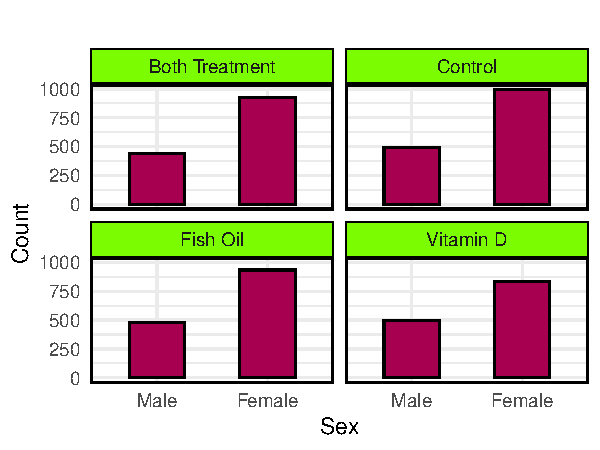
\includegraphics{Final_Report_files/figure-latex/unnamed-chunk-16-1} 

}

\caption{The distribution of age in each treatment group, which appear to be normal/ positive skewed distributions.}\label{fig:unnamed-chunk-16}
\end{figure}

\begin{figure}

{\centering 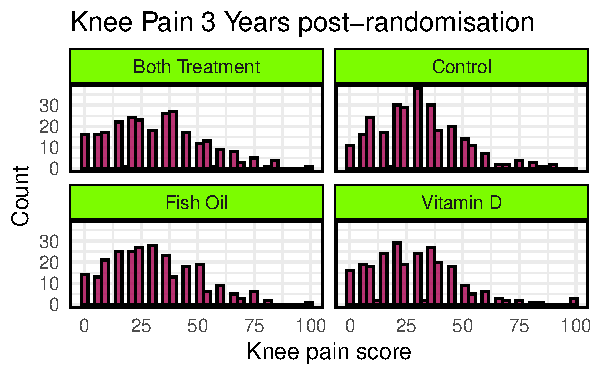
\includegraphics{Final_Report_files/figure-latex/unnamed-chunk-17-1} 

}

\caption{The distribution of body mass index in each treatment group, these appear to be positively skewed with a BMI between 20 and 40. This shows a range between healthy weighted and obese participants.}\label{fig:unnamed-chunk-17}
\end{figure}

\begin{figure}

{\centering 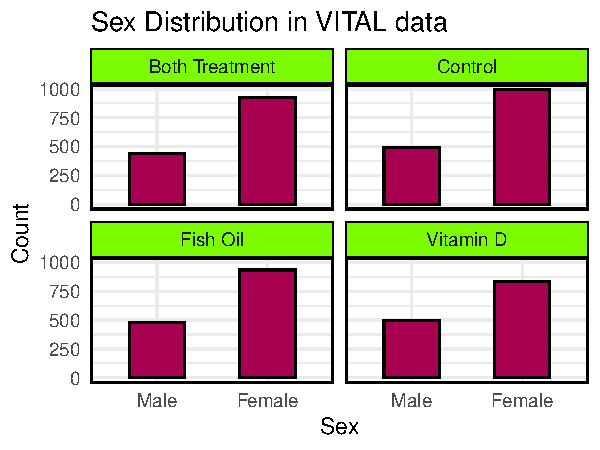
\includegraphics{Final_Report_files/figure-latex/unnamed-chunk-18-1} 

}

\caption{The distribution of males and females in the VITAL data. Similar to the acupuncture trial, the participants are predominantly female.}\label{fig:unnamed-chunk-18}
\end{figure}

\pandocbounded{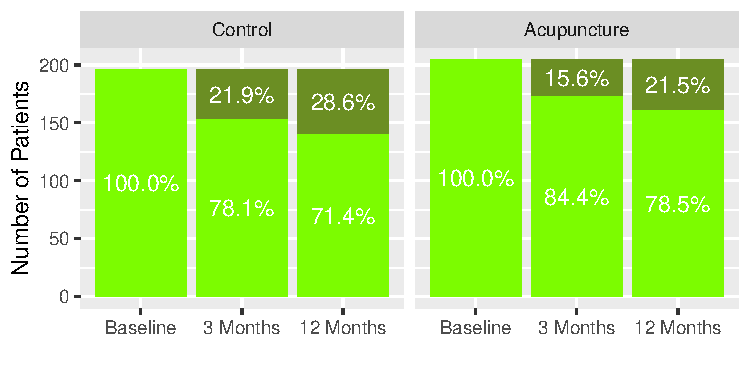
\includegraphics[keepaspectratio]{Final_Report_files/figure-latex/unnamed-chunk-19-1.pdf}}

\pandocbounded{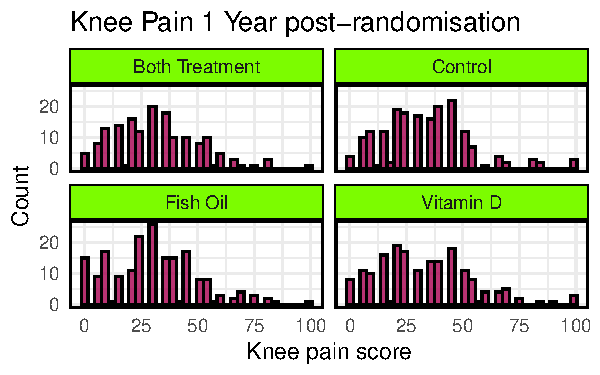
\includegraphics[keepaspectratio]{Final_Report_files/figure-latex/unnamed-chunk-20-1.pdf}}

\pandocbounded{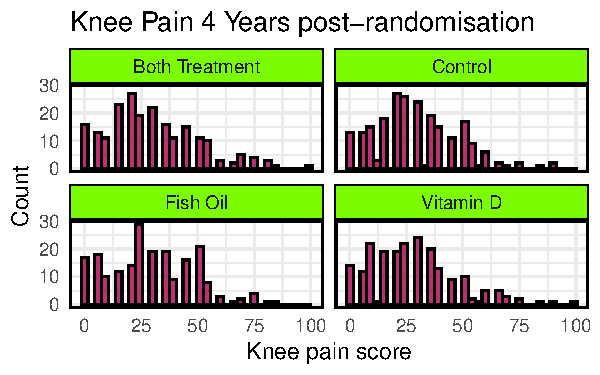
\includegraphics[keepaspectratio]{Final_Report_files/figure-latex/unnamed-chunk-21-1.pdf}}

\pandocbounded{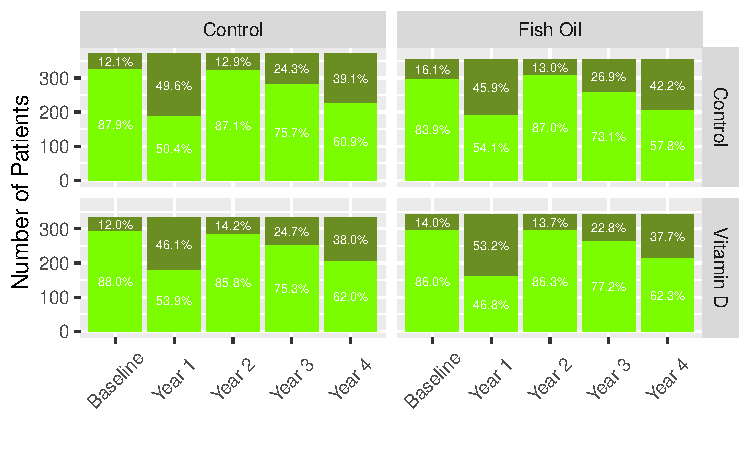
\includegraphics[keepaspectratio]{Final_Report_files/figure-latex/unnamed-chunk-22-1.pdf}}

\pandocbounded{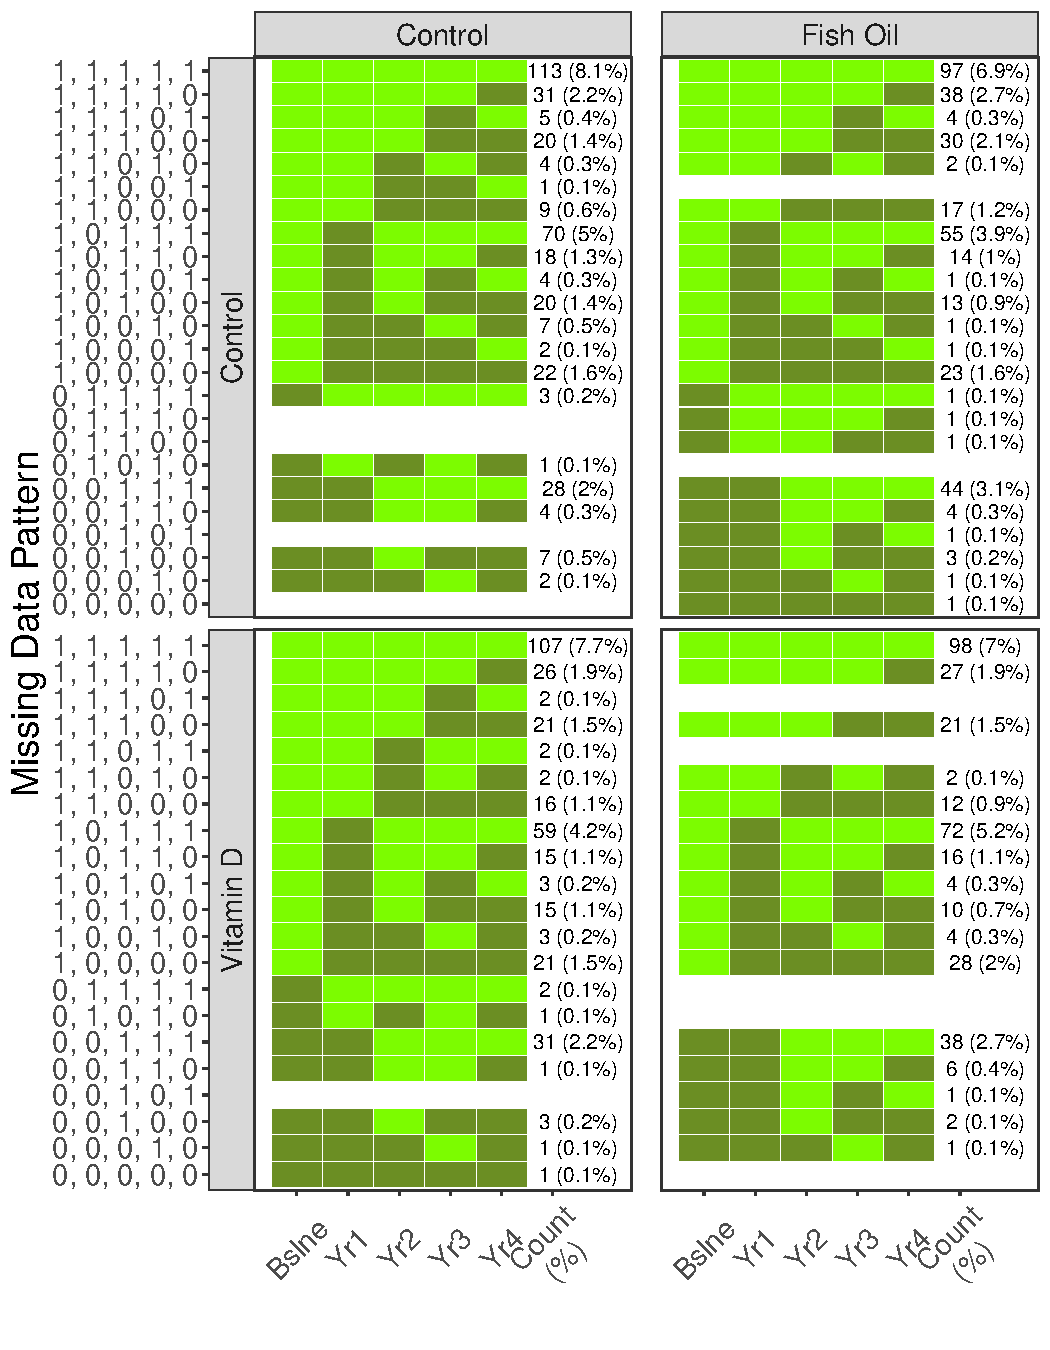
\includegraphics[keepaspectratio]{Final_Report_files/figure-latex/unnamed-chunk-23-1.pdf}}

Figure 2.x,2.x,2.x,2.x,2.x shows the distribution of the knee pain from
baseline until 4 years post randomisation. In all treatment groups it
appears that the distributions follow a positive/ near normal
distribution and skews more positive as time goes on. This occurs in all
groups. Each time-point has an incomplete distribution due to missing
data.

\newpage

\subsection{Missing analysis}\label{missing-analysis}

\textbf{Acupuncture Data}

The summary statistics of the acupuncture trial data shows that all
baseline variables have been observed. It appears two post-randomisation
outcome variables contain missing data. This pattern would be described
as a multivariate monotonic pattern as the percentage of missing data
increases at each follow up time point, which is common in longitudinal
studies. We can visualise this in the plot below.

\begin{figure}
\centering
\pandocbounded{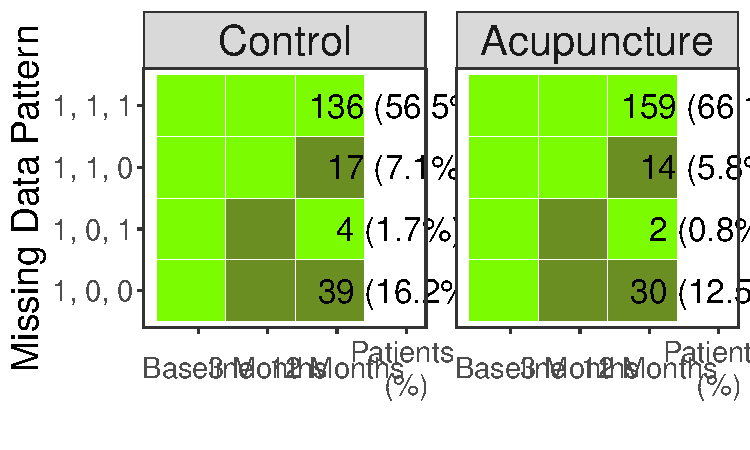
\includegraphics[keepaspectratio]{Final_Report_files/figure-latex/unnamed-chunk-24-1.pdf}}
\caption{Proportion of missing data in outcome variables \(pk2\) and
\(pk5\). This follows a monotonic missing data pattern.}
\end{figure}

If we separate the acupuncture trial data into the treatment group and
control group, we can observe that there is a higher percentage of
missing data in the control group.

\begin{figure}
\centering
\pandocbounded{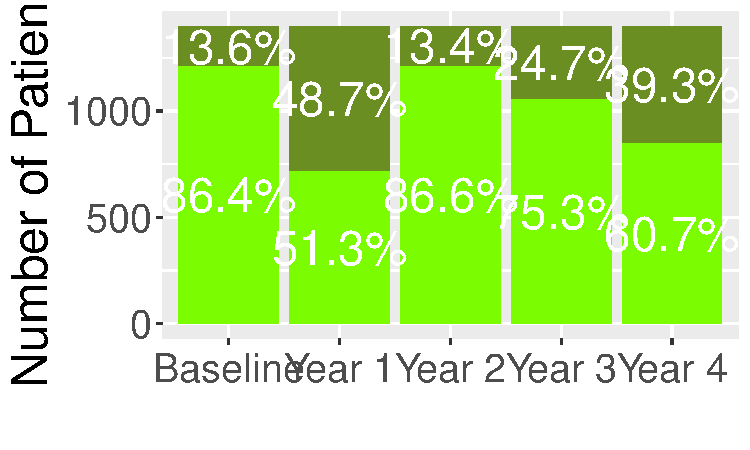
\includegraphics[keepaspectratio]{Final_Report_files/figure-latex/unnamed-chunk-25-1.pdf}}
\caption{Higher percentage of missing data (dark green) in control
group}
\end{figure}

If we investigate the missing data pattern in more detail, we can see
that the pattern is similar in both groups. In the plot below, we can
see that the pattern in which the three headache severity scores
\(pk1\), \(pk2\) and \(pk5\) are observed (1,1,1) followed by the
pattern in which both post-randomised headache severity scores contain
missing data (1,0,0).

\begin{figure}
\centering
\pandocbounded{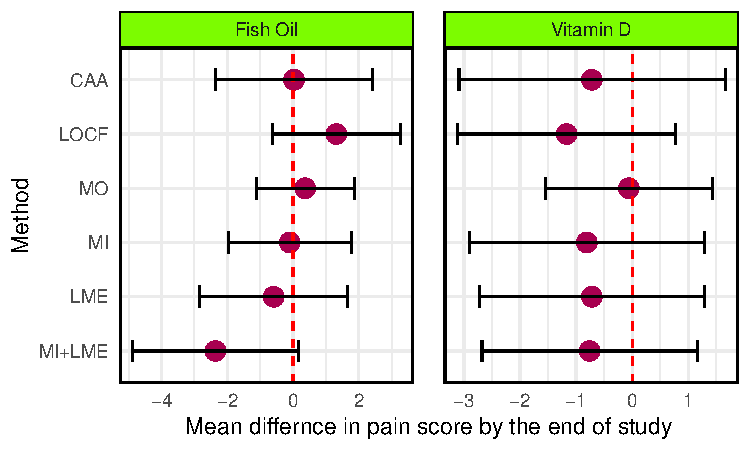
\includegraphics[keepaspectratio]{Final_Report_files/figure-latex/unnamed-chunk-26-1.pdf}}
\caption{Missing data pattern is similar in both groups (1=observed,
0=missing)}
\end{figure}

\textbf{VITAL data}

The summary statistics of the VITAL data showed, unlike the acupuncture
trial data, there are also baseline variables that contain missing data
as well as the post randomised variables. A non-monotic multivariate
pattern appears to show here as there is a great proportion of missing
data in the knee pain score at the first year post randomisation, which
drastically decreases in year 2, then steadily increases again.

\begin{figure}
\centering
\pandocbounded{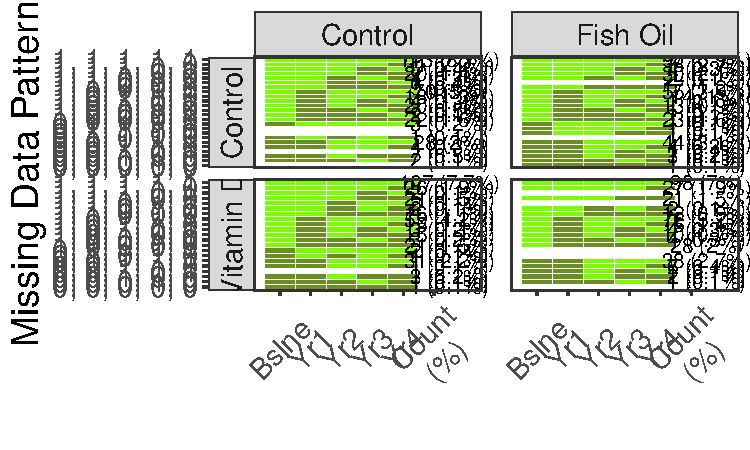
\includegraphics[keepaspectratio]{Final_Report_files/figure-latex/unnamed-chunk-27-1.pdf}}
\caption{Non-monotonic pattern across out knee pain scores in VITAL
data.}
\end{figure}

Recall that the VITAL data set contains 4 different combinations of
treatment. Separating this out in the plot below we can see the
percentage of missing data in each knee pain time point variable in each
group. The proportion appears to be similar in each group with year 2
post randomisation containing the most missing data.

\begin{figure}
\centering
\pandocbounded{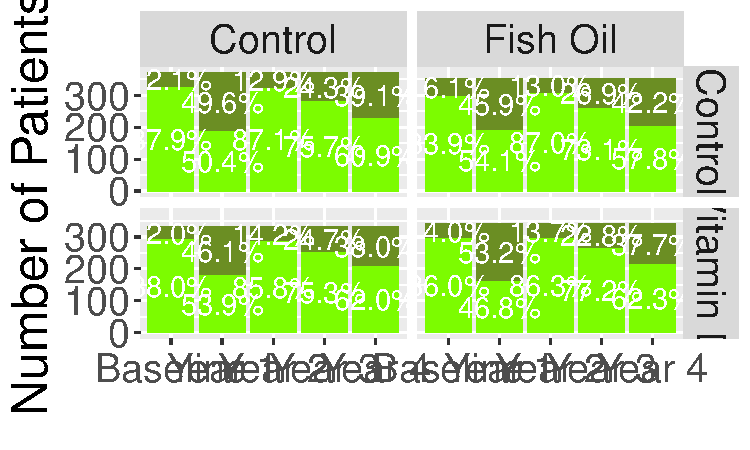
\includegraphics[keepaspectratio]{Final_Report_files/figure-latex/unnamed-chunk-28-1.pdf}}
\caption{Percentage of missing data across baseline and 4 follow-up time
points. Non-monotonic pattern appears similar in 4 randomised groups.}
\end{figure}

Looking at the possible missing data patterns in the 4 combinatory
groups, they are mostly similar with little anomalies. As this dataset
has more time-points recorded than the acupuncture trial data, and more
treatmenr groups, there are more possible missing data patterns to
observe. The most common data pattern still stands as (1,1,1,1,1) in
which data is observed at all time-points.

\begin{figure}
\centering
\pandocbounded{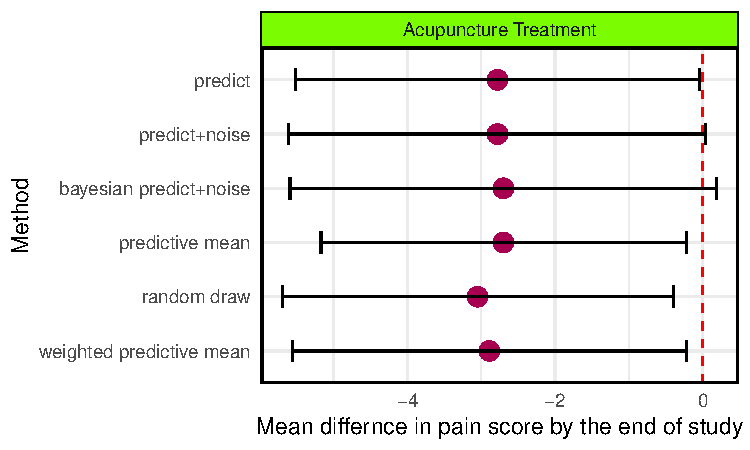
\includegraphics[keepaspectratio]{Final_Report_files/figure-latex/unnamed-chunk-29-1.pdf}}
\caption{Missing data patterns across 4 treatment groups in VITAL data.}
\end{figure}

\newpage

\section{Methods}\label{methods}

\subsection{Anchoring methods}\label{anchoring-methods}

We began our analysis with basic methods to serve as a comparison
benchmark for more advanced techniques. As previously mentioned, these
included complete case analysis, LOCF, and the mean observation method.
Each of these approaches was used to anchor the results and provide a
reference point for evaluating the performance of more robust models.

\subsubsection{Complete case analysis}\label{complete-case-analysis}

For both datasets, given that our estimand is the mean difference in
pain scores at the end of the study, we fit a model regressing the final
pain score on treatment group and baseline pain score. CCA can yield
valid inferences when the data are MCAR, or when the outcome is MAR
conditional on the variables included in the model. In our analysis, we
adjust for treatment group and baseline pain score. To ensure
comparability across methods and to reduce computational burden, we did
not include additional covariates in any of the analyses.

We applied the following models for each dataset:

\begin{Shaded}
\begin{Highlighting}[]
\CommentTok{\# For acupuncture data set}
\NormalTok{acu\_CAA }\OtherTok{\textless{}{-}} \FunctionTok{lm}\NormalTok{(pk5 }\SpecialCharTok{\textasciitilde{}}\NormalTok{ group }\SpecialCharTok{+}\NormalTok{ pk1 , }\AttributeTok{data =}\NormalTok{ acu\_wide)}
\CommentTok{\# For VITAL data set}
\NormalTok{vital\_complete }\OtherTok{\textless{}{-}} \FunctionTok{lm}\NormalTok{(pain\_yr4 }\SpecialCharTok{\textasciitilde{}}\NormalTok{ fishoilactive }\SpecialCharTok{+}\NormalTok{ vitdactive }\SpecialCharTok{+}\NormalTok{ pain\_base, }\AttributeTok{data =}\NormalTok{ vital\_wide)}
\end{Highlighting}
\end{Shaded}

One of the main drawbacks of using CCA is the loss of power due to
reduced sample size, along with the risk of introducing bias. In our
implementation, the lm() function in R automatically excludes any
individual with missing values in the model variables. As a result, we
are left with only 301 out of 401 observations in the acupuncture
dataset and 698 out of 1390 in the VITAL dataset---corresponding to a
loss of approximately 25\% and 50\% of the sample size, respectively.

We have not included many covariates in our models, so bias could exist
even with complete data due to omitted variables. Now, suppose we
attempted to adjust for all relevant baseline covariates---missing data
would still pose a problem. For instance, in the VITAL dataset, several
baseline covariates have missing values. Excluding observations with
missing data in these variables could still induce bias, particularly if
the missingness is related to the outcome.

In the acupuncture dataset, although there is no missingness in baseline
variables, CCA has further limitations. While intermediate outcomes such
as the 3-month pain score or post-randomisation variables like pain
frequency may contain valuable information, they are not included in our
models. This is not due to a limitation of CCA or LME itself, but
because including post-randomisation variables would violate the goal of
estimating the total effect of randomisation. However, these variables
can still contribute indirectly through MI. Rather than adjusting for
them in the model, MI treats repeated and related measures as part of a
multivariate distribution within each individual, allowing partially
observed variables to help impute missing values without compromising
the target estimand.

In rare cases---such as when the sole interest is in estimating the mean
difference between groups at the end of the study, and there are no
important non-baseline covariates complete case analysis can still yield
valid results. Thus when apply complete case analysis, we are assuming:
the outcome is MAR, conditional on the observed baseline predictors
included in the model.

This condition sometimes referred to as ``conditionally MCAR''. While it
is weaker than the strict MCAR assumption, it is still quite strong. It
implies that:

\begin{itemize}
\tightlist
\item
  Missingness depends only on the variables included in the model;
\item
  The model is correctly specified;
\item
  The outcome variable is not involved in the missingness
  mechanism---consistent with the MAR framework.
\end{itemize}

Under these assumptions, CCA can provide unbiased estimates. However,
they are rarely fully met in practice, especially in complex
longitudinal studies where many relevant variables and time points are
involved.

This can be expressed in the mathematics form, assuming outcome of
interest Y MAR depends on baseline covaraites X

\begin{align*}
  Pr(R_i=1 \mid Y_i, X_i) = Pr(R_i=1 \mid X_i)
  \end{align*}

Thus, we can infer under MAR, the distribution of outcome within
covaraites is the same in the observed data, the unobserved data, and
the population.

\begin{align*}
  & Pr(Y_i \mid R_i=1, X_i) \\ 
  & = \displaystyle \frac{Pr(R_i=r,Y_i,X_i)}{Pr(R_i=1,X_i)} \\
  & = \displaystyle \frac{Pr(R_i=1 \mid Y_i,X_i)Pr(Y_i,X_i)}{Pr(R_i=1 \mid X_i)Pr(X_i)} 
  \\
  & Assuming \ \ \Pr(R_i=1 \mid Y_i, X_i) = Pr(R_i=1 \mid X_i) \\
  & = \displaystyle \frac{Pr(Y_i,X_i)}{Pr(X_i)} \\
  & = Pr(Y_i \mid X_i)
  \end{align*}

The key issue is that we aim to include as much relevant information as
possible in the set of predictors X to make the MAR assumption more
plausible and robust. As discussed above, more statistically principled
methods---such as multiple imputation or mixed-effects models---allow us
to incorporate a broader set of variables and handle missingness more
effectively. However, it is important to note that the MAR assumption is
fundamentally untestable. Therefore, to assess the robustness of our
conclusions, we must perform sensitivity analyses, which are presented
in later sections.

\subsubsection{Last observation carry
forward}\label{last-observation-carry-forward}

LOCF is a simple imputation method that fills in missing values based on
the last observed outcome for each subject. It relies on assumptions
unrelated to the missing data mechanism, meaning it does not model the
reason for missingness. Instead, LOCF assumes that the outcome remains
stable after dropout, which may be plausible in some clinical contexts,
such as when the treatment effect has plateaued or when patients are
expected to remain in a steady state.

However, this assumption is not convincing in either of the datasets
analyzed here. In both the Acupuncture and VITAL trials, pain score are
unlikely to be stabilized throughout, and the outcomes display trends
over time, making the LOCF assumption potentially misleading and
unsuitable for accurate estimation of treatment effects.

\subsubsection{Mean observation method}\label{mean-observation-method}

Mean imputation is another simple method that fills in missing values by
replacing them with the mean of the observed data at each timepoint.
Like LOCF, it is based on assumptions unrelated to the missing data
mechanism and does not attempt to model why the data are missing.

This method implicitly assumes that the mean of the observed values
accurately represents the population mean, which can be problematic. In
fact, this can be viewed as an even more radical assumption than
assuming data are MCAR, since it ignores potential bias introduced by
the missingness and oversimplifies individual variation.

As with LOCF, this assumption is not convincing in either of the data
sets analyzed here. In both the Acupuncture and VITAL trials, pain
scores vary over time, and individual trajectories differ. Replacing
missing values with the average observed value at each time point
disregards this variation and may lead to underestimated variability and
biased treatment effect estimates.

\subsection{Changing imputation
methods}\label{changing-imputation-methods}

To address missing data in a statistically principled manner, it is
helpful to distinguish between two components: the imputation step and
the modeling step. In our anchoring methods, we either did not perform
imputation---as in CCA---or relied on single imputation techniques, such
as LOCF or mean imputation.

While methods like LME can utilize most available observed data and
yield unbiased estimates under the MAR assumption without imputation,
they cannot incorporate other post-randomization variables that are not
part of the model (e.g., pain frequency in the acupuncture data set). In
contrast, MI allows the inclusion of such auxiliary information during
the imputation process.

In most realistic scenarios, doing no imputation or applying single
imputation methods is likely to introduce bias and underestimate
uncertainty, especially when missingness is related to unobserved
outcomes. Thus, more flexible approaches---such as MI combined with
appropriate modeling---are generally preferred for robust inference in
the presence of missing data.

\subsubsection{Multiple imputation}\label{multiple-imputation}

A key limitation of single imputation methods is that they treat imputed
values as if they were observed data when fitting the substantive model.
This approach fails to reflect the inherent uncertainty associated with
missing values---it assumes we have perfectly recovered the unobserved
data, which is never the case in practice.

In reality, the best we can do is to estimate the distribution of the
missing data conditional on the observed data, under specific
assumptions about the missingness mechanism (e.g., MAR). Importantly,
this distribution is not adequately captured by a single draw, as is
done in single imputation. Instead, to account for uncertainty, we must
generate multiple draws from this distribution, resulting in multiple
imputed datasets. This is the foundation of Multiple Imputation (MI).

As we will demonstrate in the following sections, the draws used in MI
must be (at least approximately) Bayesian for Rubin's variance formula
to yield valid inference. By fitting the substantive model separately to
each of the K completed datasets, we obtain multiple estimates that,
when pooled, incorporate both within-imputation variability and
between-imputation variability. This approach not only addresses bias
caused by missing data but also appropriately inflates standard errors
to reflect the uncertainty introduced by imputation. Rubin's rules
provide a general framework for combining these estimates to obtain
point estimates, variances, confidence intervals, and statistical tests.

We also briefly introduce the different methods available for performing
multiple imputation (Carpenter et al. 2023). In cases with a monotonic
missing data pattern, sequential regression offers a straightforward
solution. For arbitrary or multivariate missingness, more flexible
approaches like joint modeling or Fully Conditional Specification
(FCS)---also known as multiple imputation by chained equations
(MICE)---are required.

In our project, we chose the FCS approach, given its flexibility and
ease of use when dealing with datasets like Acupuncture and VITAL that
have complex missingness patterns across multiple variables. A brief
comparison of joint modeling versus FCS is included below to justify
this decision.

While we used five imputations (K = 5) for our MI procedure in this
analysis, we also discuss the considerations involved in choosing the
number of imputations. These include factors such as the proportion of
missing data, computational cost, and the desired precision of standard
errors and confidence intervals.

\paragraph{Rubin's rules}\label{rubins-rules}

Once multiple imputed datasets are generated, Rubin's rules
(\emph{(Rubin1987) Multiple Imputation for Nonresponse in Surveys} 1987)
are used to combine the parameter estimates and associated uncertainty
across the K imputed datasets. The steps are as follows:

\begin{enumerate}
\def\labelenumi{\arabic{enumi}.}
\item
  Impute K complete datasets, each containing different plausible values
  for the missing data. (More details in later section, we will focus on
  the following steps for now)
\item
  Fit the substantive model (e.g., a linear model or mixed-effects
  model) to each imputed dataset, obtaining Parameter estimate
  \(\hat{\beta}_{k}\) and Variance estimate \(\hat{\sigma}_{k}^{2}\) for
  each k=1,2,\ldots,K
\item
  Compute the pooled estimate \(\hat{\beta}_{MI}\) and its total
  variance \(\hat{V}_{MI}\): \begin{align*}
    \hat{\beta}_{MI} = \frac{1}{K} \sum_{k=1}^{K}{\hat{\beta}_{k}} \\
    \hat{V}_{MI} = \hat{W} + (1 + \frac{1}{K}) \hat{B} \\
    \hat{W} = \frac{1}{K} \sum^{K}_{k=1}{\hat{\sigma}^{2}_{k}} \\
    \hat{B} = \frac{1}{K-1} \sum^{K}_{k=1}({\hat{\beta}_{k}} - \hat{\beta_{MI}})^{2} \\
    \end{align*}
\item
  To test a null hypothesis \(\hat{\beta}_{MI} = \beta^{0}\) use a
  t-statistic with \(\nu\) degrees of freedom. This allows us to
  construct confidence intervals and perform hypothesis testing,
  reflecting the additional uncertainty due to imputation.
  \begin{align*}
    T = \frac{\hat{\beta}_{MI} - \beta^{0}}  {\sqrt{\hat{V}_{MI}}} \\
    \nu = (K-1)[1 + \frac{\hat{W}}{(1 + 1/K) \hat{B}}]^{2}
    \end{align*}
\end{enumerate}

\paragraph{Sequential regression MI}\label{sequential-regression-mi}

In many longitudinal studies, the missing data pattern is approximately
monotonic, particularly when dropout is due to participant withdrawal, a
common situation in clinical research. In such cases, later measurements
are often missing while earlier ones are observed, which permits the use
of sequential regression for imputation under the assumption of MAR.

To justify this, consider the joint distribution of the outcome vector
for individual \(i\) can be factorized as:

\begin{align*}
    f(Y_{i,1},Y_{i,2},...,Y_{i,p}) = f(Y_{i,p} \mid Y_{i,1},...,Y_{i,p-1}) * 
    f(Y_{i,p-1} \mid Y_{i,1},...,Y_{i,p-2}) * ... * f(Y_{i,2} \mid Y_{i,1}) 
    * f(Y_{i,1})
    \end{align*}

Under a monotonic missingness pattern, for each missing value
\(Y_{i,j}\) all preceding values \(Y_{i,1},...,Y_{i,j-1}\) are observed.
If we also assume MAR, then each of these conditional distributions can
be estimated directly from the observed data. This provides a principled
basis for sequential regression imputation, where each variable is
regressed on the variables preceding it in order, and missing values are
imputed based on those conditional models.

Suppose we have \(i=1,...,n\) individual with \(j=1,...,p\) variables.
When the missing data pattern is monotonic, sequential regression
provides an efficient and valid approach to imputation under the MAR
assumption. The procedure follows these steps:

\begin{enumerate}
\def\labelenumi{\arabic{enumi}.}
\tightlist
\item
  specify the model
\end{enumerate}

\begin{align*}    
    Y_{i,j} = (1,Y_{i,1},...,Y_{i,j-1})^{T} * \beta_{j} + 
    e_{i,j},\ {e_{i,j}^{i.i.d.} \sim{N} (0,\sigma^{2}_{j})}
    \end{align*}

\begin{enumerate}
\def\labelenumi{\arabic{enumi}.}
\setcounter{enumi}{1}
\item
  Under the monotonic pattern, for every missing \(Y_{i,j}\) we assume
  that \(Y_{i,1},...,Y_{i,j-1}\) are fully observed. We fit the
  regression model using ordinary least squares (OLS) to obtain
  estimates \(\hat{\beta}_{j},\hat{\sigma}_{j}^{2}\)
\item
  To incorporate uncertainty, we draw new parameters
  \(\beta_{j}^{*},\sigma_{j}^{*2}\) from their posterior distributions:
\end{enumerate}

\begin{align*}
   \sigma_j^{*2} = \frac{\hat{\sigma}_j^2 (n_j - j)}{z} \\
   \beta^* \sim N(\hat{\beta}, \sigma_j^{*2} A_j) \\
   A_j = (\sum_{i=1}^{n_j} x_{i,j} x_{i,j}^T)^{-1}
   \end{align*}

\begin{enumerate}
\def\labelenumi{\arabic{enumi}.}
\setcounter{enumi}{3}
\item
  For individuals with missing \(Y_{i,j}\) generate imputations from the
  model:
  \(Y_{i,j} = (1,Y_{i,1},...,Y_{i,j-1}) \beta^{*} + e^{*}_{i,j}\),
  \(e_{i,j}^{*} \sim{N} (0,\sigma^{*2}_{j})\)
\item
  Repeat for \(Y_{i,j+1}\) until complete
\end{enumerate}

This sequential regression method is applicable to datasets with a
monotonic missingness pattern, such as the Acupuncture dataset, where
individuals tend to drop out in a consistent, time-ordered manner.
However, it is not suitable for datasets with non-monotonic missingness,
such as VITAL, where some individuals may have missing values at
intermediate time points but return for later follow-ups. In such cases,
more flexible approaches like Joint Modeling or FCS are required to
properly handle the complex, arbitrary missing data structure.

\paragraph{Joint modelling}\label{joint-modelling}

When the missing data pattern is non-monotonic, as in the VITAL dataset,
sequential regression is no longer appropriate. Instead, we can apply
joint modeling, which makes no assumption about the missingness pattern
but assumes the missing data mechanism is ignorable (typically, Missing
At Random).

Under joint modeling, we assume that the complete multivariate outcome
vector follows a multivariate normal distribution: \begin{align*}
    & Y \sim N(\beta,\ \Omega) \\
    & Y = (Y_{i,1},Y_{i,2},...,Y_{i,p})^{T} \\
    & \beta = (\beta_{0,1},\beta_{0,2},...,\beta_{0,p})^{T} \\
    & \Omega \ \text{is the covariance matrix}
    \end{align*}

To estimate the parameters \(\beta\) and \(\Omega\) and impute missing
values, Gibbs sampling is one of the approaches. This algorithm draws
each parameter in turn, conditional on the current values of all other
parameters and the data.

To get priors to start Gibbs sampling. We begin with initial estimates
\(\beta^{0}\) and \(\Omega^{0}\), computed from the observed data. For
each variable with missing values, we also generate an initial
imputation \(Y_{M}^{0}\) by sampling from the observed values of that
variable with replacement. This allows us to calculate initial
statistics such as \(\overline{Y}^{0}\) and and the sample covariance
matrix \(S^{0}\) (Note it also used as prior sample covariance matrix
\(S^{P}\) in each iteration)

Then, for each iteration r the following steps are performed:

\begin{enumerate}
\def\labelenumi{\arabic{enumi}.}
\item
  Draw the precision matrix (inverse
  covariance):\(\Omega^{-1,r} \sim W(n + \nu, (S_p^{-1} + S^{r-1})^{-1})\)
\item
  Draw the mean
  vector:\(\beta^{r} \sim N(\bar{Y}^{r-1}, n^{-1} \Omega^r)\)
\item
  Impute missing values:
  \(Y_{M}^{r} \sim f(Y_{M} \mid \beta^{r}, \Omega^{r}, Y_{O})\)
\item
  Update the mean and covariance estimates: \(\bar{Y}^{r}\) the mean of
  the combined imputed and observed data, and \(S^{r}\) the sum of
  squares and cross-products from the combined data
\end{enumerate}

After a sufficient number of burn-in iterations, we repeat this process
K times to generate K imputed datasets. These are then analyzed using
the substantive model of interest, and Rubin's rules are applied to pool
the results, yielding valid parameter estimates and standard errors that
account for the uncertainty due to missing data.

\paragraph{Full conditional
specification}\label{full-conditional-specification}

Fully Conditional Specification (FCS), also known as multiple imputation
by chained equations (MICE), is an extension of sequential regression
imputation that relaxes the requirement that all covariate values used
in the regressions be fully observed.

Importantly, when the missingness pattern is monotonic, FCS becomes
equivalent to the sequential regression method discussed earlier.
However, its key advantage is that it remains valid under non-monotonic
missingness, making it suitable for more general data structures like
the VITAL dataset.

The term ``full conditional specification'' refers to the fact that each
variable is imputed from its full conditional distribution, given all
other variables. This allows for more flexible modeling of multivariate
missingness.

The general procedure involves the following steps:

\begin{enumerate}
\def\labelenumi{\arabic{enumi}.}
\item
  Reorder the variables so that the overall missingness pattern is as
  close to monotonic as possible. This can improve stability and
  convergence in the imputation process.
\item
  Initialize missing values by filling in initial guesses---often by
  drawing, with replacement, from the observed values of each variable.
\item
  For each variable \(Y_{j}\)

  \begin{itemize}
  \tightlist
  \item
    Regress the observed part of \(Y_{j}\) on all other variables
    (including those with imputed values).
  \item
    Use the fitted model to impute the missing values in \(Y_{j}\),
    treating the other variables as given.
  \end{itemize}
\item
  Repeat step 3 for all variables with missing data to complete one
  cycle.
\item
  Perform multiple cycles until convergence, and then repeat the entire
  process K times to generate K imputed datasets.
\end{enumerate}

These datasets can then be analyzed with the substantive model, and the
results pooled using Rubin's rules. FCS is widely used in practice due
to its flexibility and implementation in tools like the mice package in
R.

\paragraph{FCS VS joint modelling}\label{fcs-vs-joint-modelling}

Generally, under the assumption of a multivariate normal distribution,
the joint distribution uniquely determines the full set of conditional
distributions, and vice versa. This means that, in theory, joint
modeling and fully conditional specification (FCS) are mathematically
compatible representations of the same underlying structure---provided
all models are correctly specified.

In practice, however, joint modeling using a Gibbs sampler is often
considered a more efficient algorithm. It also has the advantage of
allowing the inclusion of prior information, which can be particularly
useful when data are sparse or when integrating external knowledge into
the model. Additionally, joint modeling methods can incorporate ridge
parameters to stabilize the estimation of the covariance matrix, which
becomes important when the number of variables is large relative to the
sample size.

However, these concerns do not apply in our project, as our datasets
have moderate dimensionality and sufficient sample size. Therefore, we
opted to use Fully Conditional Specification (FCS) for multiple
imputation.

We adopted the FCS approach using the mice package in R to perform
multiple imputation throughout this project. One advantage of FCS is its
ease of implementation, as it does not require explicit specification of
a joint model or prior distributions, and it typically converges in
fewer iterations in practice. Moreover, the balanced longitudinal design
of both datasets---where follow-up measurements occur at consistent time
points across individuals---makes FCS especially suitable. This
structure allows for sequential imputation of partially observed
variables in a consistent order across patients. In contrast, if the
data were collected at irregular or patient-specific time points, or
under a more complex design such as a cluster randomised trial, the FCS
approach would be more difficult to apply reliably.

Finally, within the MICE framework, different imputation methods can be
specified for different variable types---such as predictive mean
matching or sampling from observed values. We will explore the impact of
these options later in the analysis.

\paragraph{How to choose imputation number
K}\label{how-to-choose-imputation-number-k}

Another practical consideration in multiple imputation (MI) is the
choice of the number of imputations, denoted by K. While early
applications often used K=5, more recent work emphasizes that the
optimal number depends on the degree of missing information in the data.

A key parameter in determining K is \(\gamma_{0}\), which represents the
fraction of missing information for the parameter of interest.
Unfortunately, \(\gamma_{0}\) is typically unknown in advance, including
in our project.

To address this, (White, Royston, and Wood 2011) proposed a simple and
conservative strategy: using the proportion of complete cases in the
dataset as a proxy for \(1-\gamma_{0}\), thereby estimating
\(\gamma_{0}\) conservatively. This approach allows for an informed yet
practical choice of K, especially when precise calculation of the
missing information is not feasible.

In our analysis, we used K=5 imputations as a baseline, while
recognizing that more imputations may be needed in cases with higher
levels of missingness or if more precise estimates of standard errors
are required. We will explore the implication of changing K in the
following sessions.

\textbf{Choose 3-5 imputations}

The classic advice for multiple imputation is to use a low number of
imputations, typically between 3 and 5, when the proportion of missing
information is moderate. As discussed in (\emph{(Rubin1987) Multiple
Imputation for Nonresponse in Surveys} 1987), the argument for choosing
a small K is based on the total variance
estimate:\(T_{K} = (1 + \frac{\gamma0}{K}) T_{\infty}\)

where \(T_{K}\) is the variance with K imputations, \(T_{\infty}\) is
the asymptotic variance as \(K \rightarrow \infty\) and \(\gamma_{0}\)
is the fraction of missing information. Since \(\gamma_{0}\) is
typically unknown, this formula helps illustrate the trade-off between
the number of imputations and efficiency.

There is often limited benefit in increasing K beyond 5. For instance,
if \(\gamma0=30\%\), using K = 5 result in \(T_m=1.06T_\infty\),
indicating only a 6\% inflation in variance compared to the ideal case.

In this project, we chose to use K=5 imputations for multiple
imputation, following the classical recommendation to use a low number
of imputations when the proportion of missing information is moderate.

\textbf{Chosse \textgreater20 imputations}

While early guidelines recommended using a low number of imputations
(typically K=3-5) for moderate missingness, more recent research argue
that increasing K beyond this range can yield important gains in
statistical efficiency.

\begin{itemize}
\tightlist
\item
  (Royston 2004) suggested that to constrain the coefficient of
  variation of \(ln(t_{\nu}\sqrt{T})\) to below 0.05---effectively
  keeping the width of confidence intervals within about 10\%
  uncertainty, a minimum of K\textgreater20 is required. Here,
  \(t_{\nu}\) is the quantile from a t-distribution with \({\nu}\)
  degrees of freedom, reflecting the uncertainty from finite
  imputations, and \(T\) is the total variance combining within- and
  between-imputation components.
\item
  (Graham, Olchowski, and Gilreath 2007) argued that to achieve
  statistical power within 1\% of the theoretical maximum, researchers
  should use at least K=20.
\item
  (Bodner 2008) examined how the number of imputations relates to the
  fraction of missing information \(\gamma_{0}\), and its effect on
  p-values and confidence intervals. He recommended increasing
  \(K=(3,6,12,24,59,114,258)\) for \(\gamma0=(0.1, 0.3, 0.5, 0.7, 0.9)\)
  accordingly.
\end{itemize}

In some situations---such as when estimating variance components or when
dealing with highly uncertain estimands---using a very high number of
imputations (e.g.,K=200) may be warranted to approximate the full
posterior distribution.

The main drawback of increasing K is that it leads to longer
computational time. However, this is generally the only limitation, and
it becomes manageable with modern computing resources. Moreover,
starting with a high number of imputations gives greater flexibility: we
can always test the stability or sensitivity of our results by
re-analyzing a subset of the imputations (e.g., comparing the
performance at K=5,10,20) without needing to re-run the entire
imputation process.

Thus, while K=3-5 is often sufficient under moderate missingness and
when the focus is on point estimates, using a larger K can improve
robustness in more demanding settings, with minimal trade-offs beyond
processing time.

\(K \approx 100\lambda\)

A widely cited rule of thumb proposed by (White, Royston, and Wood 2011)
recommends choosing the number of imputations based on the fraction of
incomplete cases in the dataset, denoted as \(\lambda\). Specifically,
they suggest setting:\(K \approx 100\lambda\)

This rule has become a de facto standard, particularly in medical
research, due to its simplicity and strong theoretical support. The key
idea is that the number of imputations should roughly match the
percentage of individuals with any missing data.

\begin{itemize}
\item
  The Monte Carlo error of the pooled point estimate \(\hat{\beta}\) is
  approximately 10\% of its standard error.
\item
  The Monte Carlo error of the test statistic
  \(\hat{\beta}/SE_{\hat{\beta}}\) is roughly 0.1.
\item
  The Monte Carlo error of a p-value is approximately 0.01 when the true
  p-value is 0.05.
\end{itemize}

These error bounds are typically acceptable in applied research,
ensuring stable estimates and valid inference without requiring an
excessive number of imputations.

One challenge with applying this rule arises in high-dimensional
settings, where the number of variables is large. In such cases, it is
common for a large proportion of individuals to have at least one
missing value, which can push \(\lambda\) close to 1. To address this,
it is reasonable to use the overall missing rate (i.e., total proportion
of missing cells in the dataset) as a conservative proxy for \(\lambda\)
when needed.

This rule provides a useful upper bound for choosing K, especially when
balancing the goals of statistical precision and computational
efficiency.

\subsection{Changing substantive
model}\label{changing-substantive-model}

Another important decision point in the missing data handling process is
the choice of the substantive model---the model used for the final
analysis after imputation. One natural alternative to standard multiple
linear regression is the linear mixed-effects model (LME).

As discussed earlier, LME has the advantage of leveraging all available
observed data, even in the presence of missingness. In fact, under
certain conditions, LME can yield valid inferences without requiring
multiple imputation, as long as the missingness mechanism is ignorable
(e.g., MAR) and auxiliary variables are not essential.

Moreover, even with fully observed data---either originally complete or
completed through imputation---LME remains a superior choice in many
longitudinal settings because it explicitly accounts for within-subject
correlation from repeated measurements. This leads to more accurate
estimates and better statistical efficiency than standard linear models,
which ignore the data's hierarchical structure.

In this project, we focus on multiple linear regression and LME, both of
which assume a linear relationship between covariates and the outcome.
However, when selecting a substantive model, it's important to evaluate
this assumption. In cases where linearity is questionable, alternative
models---such as polynomial regression or spline-based models---may
provide a better fit and should be considered.

An additional benefit of using LME is that it allows for flexible
modeling of time. Specifically, it enables us to treat time as a
continuous variable, rather than as a categorical factor, which can
improve interpretability and statistical power. This modeling choice
will be explored further in a later section.

\subsection{Data Wrangling}\label{data-wrangling}

Both the Acupuncture and VITAL datasets originate in wide format, where
each subject's repeated measurements are stored in separate columns.
While this format is convenient for some operations, it is not directly
compatible with LME, which require the data to be transformed into long
format---with one row per observation per time point.

In our project, both datasets have a balanced longitudinal design, with
follow-up measurements taken at regular, pre-specified intervals. This
is not always the case in real-world studies, where irregular or missing
time points can complicate analysis. The balanced structure in our data
allows for a more straightforward imputation of partially observed
follow-up outcomes using a multivariate distribution, making the MI
process more reliable and easier to implement.

To address these differing requirements, the following general approach
was used for both data sets:

\begin{enumerate}
\def\labelenumi{\arabic{enumi}.}
\tightlist
\item
  Perform MI in wide format using the \texttt{mice()} function, treating
  the repeated measures as separate but related variables.
\item
  Convert the imputed wide data sets to long format, which allows time
  to be included as a continuous variable in the LME model.
\item
  Fit LME models on the long-format data to model outcome trajectories
  over time while appropriately accounting for missing values and
  repeated measures.
\end{enumerate}

This strategy allows us to use multiple imputation methods compatible
with the multivariate normal assumption across time points, while still
leveraging the advantages of LME models in the analysis stage.

The balanced longitudinal design of both studies further supports this
approach: each subject was planned to have the same number of repeated
measurements at roughly equal intervals (monthly in the Acupuncture
study and yearly in the VITAL study). This regular measurement structure
allows partially observed follow-up outcomes to be imputed more reliably
using a multivariate framework.

Below is a simple schematic to illustrate the reshaping process. Here,
\texttt{Outcome1/2/3} represent repeated outcomes across three
timepoints, and \texttt{x} indicates a missing value:

\textbf{Original data (wide format):}

\begin{longtable}[]{@{}llll@{}}
\toprule\noalign{}
ID & Outcome1 & Outcome2 & Outcome3 \\
\midrule\noalign{}
\endhead
\bottomrule\noalign{}
\endlastfoot
1001 & 2.5 & 3.5 & x \\
1002 & 4.5 & x & 6.3 \\
1003 & 3.3 & 6.2 & 8.1 \\
\end{longtable}

\textbf{Completed data after multiple imputation (still wide format):}

\begin{longtable}[]{@{}llll@{}}
\toprule\noalign{}
ID & Outcome1 & Outcome2 & Outcome3 \\
\midrule\noalign{}
\endhead
\bottomrule\noalign{}
\endlastfoot
1001 & 2.5 & 3.5 & 4.5 \\
1002 & 4.5 & 5.2 & 6.3 \\
1003 & 3.3 & 6.2 & 8.1 \\
\end{longtable}

\textbf{Transformed data (long format):}

\begin{longtable}[]{@{}lll@{}}
\toprule\noalign{}
ID & Time & Outcome \\
\midrule\noalign{}
\endhead
\bottomrule\noalign{}
\endlastfoot
1001 & 1 & 2.5 \\
1001 & 2 & 3.5 \\
1001 & 3 & 4.5 \\
1002 & 1 & 4.5 \\
1002 & 2 & 5.2 \\
1002 & 3 & 6.3 \\
1003 & 1 & 3.3 \\
1003 & 2 & 6.2 \\
1003 & 3 & 8.1 \\
\end{longtable}

\subsection{Examing using forest plot}\label{examing-using-forest-plot}

To visually compare how our estimand (treatment effect) changes across
different missing data methods, we present results using a series of
forest plots. These plots allow us to directly assess the impact of each
imputation or modeling strategy on the estimated effect and its
confidence interval.

The same process was applied to both the Acupuncture and VITAL datasets.
For the VITAL trial, which follows a 2×2 factorial design, we simplify
the analysis---as previously discussed---by treating fish oil and
vitamin D as if they were tested in two separate randomized controlled
trials. This means we ignore potential interaction effects between the
two treatments and estimate their effects independently, which allows
for a more straightforward comparison across methods.

\subsubsection{Change imputation method and substantive
model}\label{change-imputation-method-and-substantive-model}

We evaluated the impact of missing data by systematically varying both
the imputation method and the substantive model used in the analysis. By
doing that, we try to isolate the effects of changing either the
imputation strategy or the analysis model, and highlights the practical
impact of each decision on the resulting treatment effect estimates.

First, as described earlier, we applied three anchoring methods:
Complete Case Analysis (CAA), Last Observation Carried Forward (LOCF),
and mean imputation. Each was followed by multiple linear regression to
estimate the treatment effect.

Next, we performed Multiple Imputation (MI) using the predictive mean
matching method with 5 imputations, again analyzing the imputed datasets
using multiple linear regression---maintaining consistency with the
anchoring models for fair comparison.

Then, we changed the substantive model to a linear mixed-effects model
(LME), without performing any imputation. This approach uses all
available observed data and accounts for repeated measurements, offering
a more efficient use of the data under the MAR assumption.

Finally, we combined both improvements: we performed MI using predictive
mean matching with 5 imputations, and analyzed the completed datasets
using the LME model.

\subsubsection{Change estimand}\label{change-estimand}

Assuming our primary objective remains to estimate the mean difference
in pain scores at the final timepoint for both datasets, we now explore
how this estimand can be more efficiently estimated by incorporating
interim outcome data.

In the previous section, we applied six different methods, two of which
used Linear Mixed-Effects (LME) models as the substantive model.
However, in those implementations, time was treated as a categorical
variable. This approach limited our ability to take full advantage of
the repeated measures structure, as it did not model the underlying
trajectory of pain over time.

To address this, we revise the estimand by treating time as a continuous
variable. This allows us to model individual pain trajectories across
the study period, thereby leveraging all available interim outcome data.
As a result, we improve the precision of the estimated treatment effect
at the final timepoint---even in the presence of missing data.

\paragraph{Original Estimand (Categoricl
Time)}\label{original-estimand-categoricl-time}

\emph{Acupuncture data set}

The goal of the original acupuncture study was to estimate the effect of
acupuncture therapy versus general care on chronic headache severity.
The estimand of interest is the mean difference in headache scores at 12
months, conditional on baseline severity. This can be expressed with the
following linear regression model:

\[pk5_i = \beta_0 + \beta_1 group_i + \beta_2 pk1_i + \varepsilon_i\]
where

\begin{itemize}
\tightlist
\item
  \(pk5_i\): headache pain score of individual \(i\) at 12 months.
\item
  \(pk1_i\): adjusted baseline headache pain score of individual \(i\)
\item
  \(group_i\): binary indicator of treatment assignment (1 =
  acupuncture, 0 = control)
\item
  \(\beta_0\): intercept, representing the expected 12-month pain score
  for a control participant with zero baseline pain
\item
  \(\beta_1\): treatment effect of acupuncture relative to control; this
  is the estimand of interest
\item
  \(\beta_2\): effect of baseline headache severity on the 12-month
  outcome
\item
  \(\varepsilon_i\): residual error term for individual \(i\)
\end{itemize}

\emph{VITAL data set}

In the VITAL study, the primary aim was to evaluate the effects of
vitamin D and fish oil supplementation on knee pain four years after
randomisation. The estimand of interest is the mean difference in knee
pain scores at 4 years, conditional on baseline pain. This is modelled
using the following linear regression:

\[painyear4_i = \beta_0 + \beta_1 fishoilactive_i + \beta_2 vitdactive_i + \beta_3 painbase_i + \varepsilon_i\]

where

\begin{itemize}
\tightlist
\item
  \(pain_yr4_i\): knee pain score for individual \(i\) at 4 years
  post-randomization
\item
  \(fishoilactive_i\): binary indicator for fish oil treatment (1 =
  active, 0 = placebo)
\item
  \(vitdactive_i\): binary indicator for vitamin D treatment (1 =
  active, 0 = placebo)
\item
  \(painbase_i\): baseline knee pain score for individual \(i\)
\item
  \(\beta_0\): intercept, representing the expected 4-year pain score
  for a participant receiving neither treatment and with zero baseline
  pain
\item
  \(\beta_1\): effect of fish oil supplementation; this is the estimand
  of interest in the fish oil analysis
\item
  \(\beta_2\): effect of vitamin D supplementation; this is the estimand
  of interest in the vitamin D analysis
\item
  \(\beta_3\): effect of baseline pain on the 4-year outcome
\item
  \(\varepsilon\): residual error term for individual \(i\)
\end{itemize}

\paragraph{Changed Estimand (Continuous
Time)}\label{changed-estimand-continuous-time}

To better utilise repeated measures in both datasets, we revise the
estimand using a Linear Mixed-Effects (LME) model with time treated as a
continuous variable.

To ensure that the intercept represents the estimated treatment effect
specifically at the end of follow-up, we re-center the time variable: -
In the acupuncture study, we define \(time_c = time - 12\) (in months),
so that time zero corresponds to month 12, which is the end of study. -
In the VITAL study, we define \(time_{contin} = time - 4\) (in years),
so that time zero corresponds to year 4, which is the end of study.

With this centering, the model intercept represents the mean pain score
at the end of the study, and the coefficient for the treatment group
becomes the estimand of interest.

\emph{Acupuncture data set}

The revised LME model for the acupuncture dataset is specified as below.
Note we did not allowing random slop as there are only 2 data collecting
time points here:

\[
pk5_{ij} = \beta_0 + \beta_1 group_i + \beta_2 time_{c,ij} + \beta_3 (group_i \times time_{c,ij}) + \beta_4 pk1_i + b_{0i} + \varepsilon_{ij}
\]

where

\begin{itemize}
\tightlist
\item
  \(pk5_{ij}\): headache pain score for individual \(i\) at time \(j\)
\item
  \(group_i\): binary indicator of treatment assignment (1 =
  acupuncture, 0 = control)
\item
  \(time_{c,ij}\): time in months since baseline, centered at 12 months
  (\(time_c = time - 12\))
\item
  \(pk1_i\): adjusted baseline headache pain score of individual \(i\)
\item
  \(\beta_0\): intercept, representing the expected pain score at 12
  months (end of study) for the control group with zero baseline pain
\item
  \(\beta_1\): treatment effect of acupuncture relative to control at 12
  months; this is the estimand of interest
\item
  \(\beta_2\): average rate of change in pain over time in the control
  group
\item
  \(\beta_3\): treatment-time interaction effect
\item
  \(\beta_4\): effect of baseline headache pain
\item
  \(b_{0i}\): random intercept for individual \(i\)
\item
  \(\varepsilon_{ij}\): residual error term for individual \(i\) at time
  \(j\)
\end{itemize}

\emph{VITAL data set}

The revised LME model for the VITAL dataset is specified as:

\[
pain_{ij} = \beta_0 + \beta_1 fishoilactive_i + \beta_2 vitdactive_i + \beta_3 time_{contin,ij} + \beta_4 (fishoilactive_i \times time_{contin,ij}) + \beta_5 (vitdactive_i \times time_{contin,ij}) + \beta_6 painbase_i + b_{0i} + b_{1i} time_{contin,ij} + \varepsilon_{ij}
\]

where

\begin{itemize}
\tightlist
\item
  \(pain_{ij}\): knee pain score for individual \(i\) at time \(j\)
\item
  \(fishoilactive_i\): binary indicator for fish oil treatment (1 =
  active, 0 = placebo)
\item
  \(vitdactive_i\): binary indicator for vitamin D treatment (1 =
  active, 0 = placebo)
\item
  \(time_{contin,ij}\): time in years since baseline, centered at 4
  years (\(time_{contin} = time - 4\))
\item
  \(painbase_i\): baseline knee pain score for individual \(i\)
\item
  \(\beta_0\): intercept, representing the expected pain score at 4
  years (end of study) for a participant receiving neither treatment and
  with zero baseline pain
\item
  \(\beta_1\): effect of fish oil at 4 years; this is the estimand of
  interest in the fish oil analysis
\item
  \(\beta_2\): effect of vitamin D at 4 years; this is the estimand of
  interest in the vitamin D analysis
\item
  \(\beta_3\): average rate of change in pain over time in the placebo
  group
\item
  \(\beta_4\): fish oil-time interaction effect
\item
  \(\beta_5\): vitamin D-time interaction effect
\item
  \(\beta_6\): effect of baseline knee pain
\item
  \(b_{0i}\): random intercept for individual \(i\)
\item
  \(b_{1i}\): random slope for time for individual \(i\)
\item
  \(\varepsilon_{ij}\): residual error term for individual \(i\) at time
  \(j\)
\end{itemize}

\subsubsection{Change FSC methods}\label{change-fsc-methods}

Even within the FCS (Fully Conditional Specification) framework, there
are multiple imputation strategies we can explore. We begin with
deterministic prediction (method=``norm.predict''), which imputes
missing values using predicted values from a linear regression model.
Since no uncertainty is added, this is not technically multiple
imputation---each missing value is replaced by a single fixed estimate.

To account for uncertainty in the outcome, we adds random noise to the
regression prediction (method=``norm.nob''). Further, to reflect
uncertainty in the model parameters, norm draws both regression
coefficients and residual variance from their posterior distributions,
providing a fully Bayesian imputation (method=``norm'').

Alternatively, instead of model-based predictions, we can impute using
observed values. predictive mean matching (method=``pmm'') selects donor
values from observed data that are closest in predicted value to the
missing case. Weighted predictive mean matching (method=``midastouch'')
extends this by weighting the distance between predicted values,
offering a more robust variant of PMM.

Or even, if we prefer a non-parametric imputation approach, we can use
the methods like random sampling (method=``sample''), which imputes
missing values by randomly sampling from the observed values of the same
variable. This method does not rely on any model or predictor variables,
and instead preserves the marginal distribution of the variable.

\subsubsection{Change imputation
numbers}\label{change-imputation-numbers}

As discussed above, there are various arguments for choosing a higher
number of imputations based on the fraction of missing information and
the desired precision of inference. To explore the impact of increasing
K, we adjusted the number of imputations accordingly in both datasets.

For the Acupuncture dataset, where approximately 25\% of cases have
missing data, we increased K from the default 5 to 20 and 25. For the
VITAL dataset, which has around 50\% missingness, we increased K from 5
to 20 and then to 50.

\subsubsection{Sensitive analysis}\label{sensitive-analysis}

As mentioned in our introduction, missing data mechanisms are
unverifiable. While it is most common to assume that data are MAR, in
reality, the mechanism could fall under MNAR. We conducted a sensitivity
analysis to assess the robustness of the estimated treatment effect
under alternative missingness assumptions. Sensitivity analysis is
recommended by the National Research Council (2010) as a best practice
for handling missing data; however, it is rarely conducted in practice.
This may reflect an underappreciation of the impact of missing data in
many studies, as well as the complexity and specialised expertise
required to perform such analyses.

A systematic review by Fiero et al.~(2016) examined 86 cluster
randomised trials published between 2013 and 2014. Among the 80 trials
that reported missing outcome data, only 14 (18\%) reported conducting a
sensitivity analysis.

In our study, we implemented multiple imputation with \(\delta\)
-adjustment as our sensitivity analysis approach. In this method, a
constant shift \(\delta\) is added to the imputed values after the
initial imputation step. This enables us to explore a range of plausible
scenarios by re-estimating the treatment effect under different
assumptions about the missing data mechanism. By applying these shift
parameters, we can model situations in which participants with missing
data are assumed to have systematically better or worse outcomes than
those observed, thereby testing the stability of our conclusions when
relaxing the MAR assumption.

The shift can be broken down in to:

\[\delta = \delta_\mathrm{MAR} + \delta_\mathrm{MNAR}\] where; -
\(\delta_\mathrm{MAR}\): mean difference caused by the predictors in the
imputation models - \(\delta_\mathrm{MNAR}\): mean difference caused by
an additional non-ignorable part of the imputation model

Essentially, \(\delta\) is the mean difference between the imputed
values and the true values that we did not observe.

Deciding which \(\delta\) values are suitable is subjective. We need to
include \(\delta\) = 0 as that assumes the data is MAR which acts as our
baseline, and we add the non-zero \(\delta\) values to test the
sensitivity to the MNAR assumption. We decided to base our \(\delta\)
values on the standard deviations of the outcome variables of interest.
The standard deviation of the headache severity score at the final time
point in the treatment group is \emph{13.71828} and \emph{17.01089} in
the control group. The standard deviation of the knee pain score at the
final time point in the fishoil group is \emph{19.13955},
\emph{19.24856} in the vitamin D group, and \emph{18.29479} in the
control group. These statistics are based on the data in the original
wide format. We also extracted the standard deviation of the outcome
variables in the long format in which the estimand is continous. We
decided an increasing and decreasing multiples of these values should
suffice;

\(\delta\) = -0.5\emph{SD, -0.25}SD, 0 , 0.25\emph{SD, 0.5}SD\$

Applying these to both datasets, our chosen \(\delta\) values are;

\emph{Original Estimand} -
\(\delta_\mathrm{Acupuncture-original} = -6.859139,-3.429569,0,3.429569,6.859139\)
-
\(\delta_\mathrm{Acu-control-original} = -8.505446,-4.252723,0,4.252723,8.505446\)
-
\(\delta_\mathrm{VITAL-fishoil-original} = -9.569774,-4.784887,0,4.784887,9.569774\)
-
\(\delta_\mathrm{VITAL-vitd-original} = -9.624281,-4.812141,0,4.812141,9.624281\)
-
\(\delta_\mathrm{VITAL-control-original} = -9.147397,-4.573698,0,4.573698,9.147397\)

\emph{Changed Estimand} -
\(\delta_\mathrm{Acupuncture-changed} = -7.397829,-3.698915,0,3.698915,7.397829\)
-
\(\delta_\mathrm{Acu-control-changed} = -8.660196,-4.330098,0, 4.330098,8.660196\)
-
\(\delta_\mathrm{VITAL-fishoil-changed} = -9.783807,-4.891904,0,4.891904,9.783807\)
-
\(\delta_\mathrm{VITAL-vitd-changed} = -9.967777,-4.983889,0,4.983889,9.967777\)
-
\(\delta_\mathrm{VITAL-control-changed} = -9.646493,-4.823247,0, 4.823247,9.646493\)

\textbf{Sensitivity Analysis; the process}

The mice() function was used on the wide format of the acupuncture trial
data with predictors \texttt{group}, \texttt{pk1}. An initial iteration
was conducted with m=1 in order to extract the post processing command.
This allows us to add the \(\delta\) to the missing values after they
have been imputed. This is looped over the range of \(\delta\) values.

Next we performed the main imputation, indicating post processing, using
predictive mean matching method and maxit=10 to indicate maximum of 10
iterations. After imputation, a regression model like our substantive
model is fitted, \(\beta_0 + \beta_1group+\beta_2pk1_i+\varepsilon_i\),
and the estimates are pooled together.

\newpage

\begin{Shaded}
\begin{Highlighting}[]
\CommentTok{\#predictors}
\NormalTok{inlist }\OtherTok{\textless{}{-}} \FunctionTok{c}\NormalTok{(}\StringTok{"group"}\NormalTok{, }\StringTok{"pk5"}\NormalTok{, }\StringTok{"pk1"}\NormalTok{)}
\CommentTok{\#predictor matrix}
\NormalTok{pred\_cat }\OtherTok{\textless{}{-}} \FunctionTok{quickpred}\NormalTok{(acu\_wide, }\AttributeTok{minpuc =} \FloatTok{0.5}\NormalTok{, }\AttributeTok{include =}\NormalTok{ inlist)}
\CommentTok{\#initial imputation to extract post processing }
\NormalTok{imp.default\_cat }\OtherTok{\textless{}{-}} \FunctionTok{mice}\NormalTok{(acu\_wide, }\AttributeTok{m =} \DecValTok{1}\NormalTok{, }\AttributeTok{maxit =} \DecValTok{1}\NormalTok{, }\AttributeTok{predictorMatrix =}\NormalTok{ pred\_cat, }\AttributeTok{seed =} \DecValTok{123}\NormalTok{, }\AttributeTok{print=} \ConstantTok{FALSE}\NormalTok{)}
\NormalTok{post\_cat }\OtherTok{\textless{}{-}}\NormalTok{ imp.default\_cat}\SpecialCharTok{$}\NormalTok{post}
\NormalTok{imp.all.undamped\_cat }\OtherTok{\textless{}{-}} \FunctionTok{vector}\NormalTok{(}\StringTok{"list"}\NormalTok{, }\FunctionTok{length}\NormalTok{(delta\_acu))}

\CommentTok{\#loop over delta values}
\ControlFlowTok{for}\NormalTok{ (i }\ControlFlowTok{in} \DecValTok{1}\SpecialCharTok{:}\FunctionTok{length}\NormalTok{(delta)) \{}
\NormalTok{  d }\OtherTok{\textless{}{-}}\NormalTok{ delta[i]}
\NormalTok{  cmd }\OtherTok{\textless{}{-}} \FunctionTok{paste0}\NormalTok{(}
    \StringTok{"idx \textless{}{-} which(data[,\textquotesingle{}group\textquotesingle{}] == 1 \& is.na(data[,\textquotesingle{}pk5\textquotesingle{}])); "}\NormalTok{,}
    \StringTok{"imp[[j]]$pk5[idx] \textless{}{-} imp[[j]]$pk5[idx] + "}\NormalTok{,d, }\StringTok{";"}\NormalTok{) }\CommentTok{\#treatment group and imputing pk5, adding delta d}
\NormalTok{  post\_cat[}\StringTok{"pk5"}\NormalTok{] }\OtherTok{\textless{}{-}}\NormalTok{ cmd}
\NormalTok{  imp\_cat }\OtherTok{\textless{}{-}} \FunctionTok{mice}\NormalTok{(acu\_wide, }\AttributeTok{pred =}\NormalTok{ pred\_cat, }\AttributeTok{post =}\NormalTok{ post\_cat, }\AttributeTok{maxit =} \DecValTok{10}\NormalTok{,}
                  \AttributeTok{seed =}\NormalTok{ i }\SpecialCharTok{*} \DecValTok{22}\NormalTok{, }\AttributeTok{print=}\ConstantTok{FALSE}\NormalTok{)}
\NormalTok{  imp.all.undamped\_cat[[i]] }\OtherTok{\textless{}{-}}\NormalTok{ imp\_cat}
\NormalTok{\}}
\NormalTok{delta\_results\_cat }\OtherTok{\textless{}{-}} \FunctionTok{data.frame}\NormalTok{()}

\ControlFlowTok{for}\NormalTok{ (i }\ControlFlowTok{in} \FunctionTok{seq\_along}\NormalTok{(imp.all.undamped\_cat)) \{}
\NormalTok{  imp\_cat }\OtherTok{\textless{}{-}}\NormalTok{ imp.all.undamped\_cat[[i]]}
\NormalTok{  d }\OtherTok{\textless{}{-}}\NormalTok{ delta[i]}
\NormalTok{  fit\_cat }\OtherTok{\textless{}{-}} \FunctionTok{with}\NormalTok{(imp\_cat, }\FunctionTok{lm}\NormalTok{(pk5 }\SpecialCharTok{\textasciitilde{}}\NormalTok{ group }\SpecialCharTok{+}\NormalTok{ pk1)) }\CommentTok{\#imputation model}
\NormalTok{  pooled\_cat }\OtherTok{\textless{}{-}} \FunctionTok{pool}\NormalTok{(fit\_cat) }\CommentTok{\#pooling estimates}
\NormalTok{  est\_cat }\OtherTok{\textless{}{-}} \FunctionTok{tidy}\NormalTok{(pooled\_cat, }\AttributeTok{conf.int =} \ConstantTok{TRUE}\NormalTok{) }\SpecialCharTok{\%\textgreater{}\%}
    \FunctionTok{filter}\NormalTok{(term }\SpecialCharTok{==} \StringTok{"group"}\NormalTok{) }\SpecialCharTok{\%\textgreater{}\%} 
    \FunctionTok{select}\NormalTok{(estimate, std.error, conf.low, conf.high, p.value) }\SpecialCharTok{\%\textgreater{}\%}
    \FunctionTok{mutate}\NormalTok{(}\AttributeTok{delta\_acu =}\NormalTok{ d)}
    
\NormalTok{  delta\_results\_cat }\OtherTok{\textless{}{-}} \FunctionTok{bind\_rows}\NormalTok{(delta\_results\_cat, est\_cat)}
\NormalTok{\}}
\end{Highlighting}
\end{Shaded}

We repeated this process exactly on the \texttt{acu\_wide} data in which
we added a filter(group==0) in order to extract the results in the
control group for comparison, creating \texttt{acu\_wide\_placebo}.

A similar process was implemented on to the VITAL trial data in wide
format. We chose our inlist predictors \texttt{pain\_base},
\texttt{vitdactive},\texttt{fishoilactive}, and our outcome as
\texttt{pain\_yr4}. After pooling our estimates, we filtered out the
treatment groups by setting `term == fishoilactive' and `term ==
vitdactive' so we can observe the results by treatment. For the control
group we filtered the \texttt{vital\_wide} data as fishoilactive==0 and
vitdactive==0.

We performed sensitivity analysis in a similar fashion to test the
robustness of the treatment effect on our alternative estimand. This was
more intensive as we had to implement the multiple imputation on the
wide format then transform the data in to long format.

For the acupuncture trial; we used our
to\_long\_format\_acu\_cont\_MICE() function post imputation to
transform to long format. Due to the nature of the long format, we used
the linear mixed effects model to estimate our treatment effect before
pooling the estimates. Our imputation model here is;

\(\text{pk\_score}_{ij} = \beta_0 + \beta_1 \text{group} + \beta_2  \text{time\_c} + \beta_3  (\text{group}  \text{time\_c}) + \beta_4  \text{pk1} + b_0 + \varepsilon_{ij}\)

\newpage

For the VITAL data; we created a similar function to our
to\_long\_format\_vital\_MICE() function with a minor adjustment;

\begin{Shaded}
\begin{Highlighting}[]
\NormalTok{to\_long\_format\_vital\_mice\_SA }\OtherTok{\textless{}{-}} \ControlFlowTok{function}\NormalTok{(data\_wide) \{}
\NormalTok{  data\_wide }\SpecialCharTok{\%\textgreater{}\%}
    \FunctionTok{pivot\_longer}\NormalTok{(}\AttributeTok{cols =} \FunctionTok{matches}\NormalTok{(}\StringTok{"\_yr[[:digit:]]$"}\NormalTok{),}
                 \AttributeTok{names\_to =} \FunctionTok{c}\NormalTok{(}\StringTok{".value"}\NormalTok{, }\StringTok{"time"}\NormalTok{), }
                 \AttributeTok{names\_sep =} \StringTok{"\_"}\NormalTok{) }\SpecialCharTok{\%\textgreater{}\%}
    \FunctionTok{group\_by}\NormalTok{(.imp) }\SpecialCharTok{\%\textgreater{}\%}
    \FunctionTok{mutate}\NormalTok{(}\AttributeTok{.id =} \DecValTok{1}\SpecialCharTok{:}\FunctionTok{n}\NormalTok{()) }\SpecialCharTok{\%\textgreater{}\%}
    \FunctionTok{mutate}\NormalTok{(}\AttributeTok{time\_contin =} \FunctionTok{as.integer}\NormalTok{(}\FunctionTok{gsub}\NormalTok{(}\StringTok{"yr"}\NormalTok{, }\StringTok{""}\NormalTok{, time)),}
           \AttributeTok{time\_contin\_cent =}\NormalTok{ time\_contin }\SpecialCharTok{{-}} \DecValTok{4}\NormalTok{)}
\NormalTok{\}}
\end{Highlighting}
\end{Shaded}

We used
\(pain_{ij}=\beta_0+\beta_1fishoil_i+\beta_2time_{ij}+\beta_3(fishoil_itime_{ij})+\beta_4vitd_i+\beta_5vitd_itime_{ij}+\beta_6(pain_base)_i+b_{0i}+\varepsilon_{ij}\)
as our imputation model in each of the imputed data sets.

\begin{Shaded}
\begin{Highlighting}[]
\CommentTok{\#predictors}
\NormalTok{inlist }\OtherTok{\textless{}{-}} \FunctionTok{c}\NormalTok{(}\StringTok{"fishoilactive"}\NormalTok{, }\StringTok{"vitdactive"}\NormalTok{, }\StringTok{"pain"}\NormalTok{, }\StringTok{"pain\_base"}\NormalTok{, }\StringTok{"time\_contin"}\NormalTok{, }\StringTok{"Subject\_ID"}\NormalTok{) }
\NormalTok{pred\_cont }\OtherTok{\textless{}{-}} \FunctionTok{quickpred}\NormalTok{(vital\_wide, }\AttributeTok{minpuc =} \FloatTok{0.5}\NormalTok{, }\AttributeTok{include =}\NormalTok{ inlist) }\CommentTok{\#prediction matrix}
\NormalTok{imp.all.undamped\_cont }\OtherTok{\textless{}{-}} \FunctionTok{vector}\NormalTok{(}\StringTok{"list"}\NormalTok{, }\FunctionTok{length}\NormalTok{(delta\_vital))}
\NormalTok{delta\_results\_cont\_fishoil }\OtherTok{\textless{}{-}} \FunctionTok{data.frame}\NormalTok{()}

\ControlFlowTok{for}\NormalTok{ (i }\ControlFlowTok{in} \FunctionTok{seq\_along}\NormalTok{(delta\_vital)) \{}
\NormalTok{  d }\OtherTok{\textless{}{-}}\NormalTok{ delta\_vital[i]}
\NormalTok{  imp\_init }\OtherTok{\textless{}{-}} \FunctionTok{mice}\NormalTok{(vital\_wide, }\AttributeTok{m =} \DecValTok{5}\NormalTok{, }\AttributeTok{maxit =} \DecValTok{1}\NormalTok{, }\AttributeTok{predictorMatrix =}\NormalTok{ pred\_cont, }\AttributeTok{seed =} \DecValTok{100} \SpecialCharTok{+}\NormalTok{ i, }\AttributeTok{print =} \ConstantTok{FALSE}\NormalTok{)}
\NormalTok{  post\_cont }\OtherTok{\textless{}{-}}\NormalTok{ imp\_init}\SpecialCharTok{$}\NormalTok{post}
\NormalTok{  method\_cont }\OtherTok{\textless{}{-}}\NormalTok{ imp\_init}\SpecialCharTok{$}\NormalTok{method}
\NormalTok{  years }\OtherTok{\textless{}{-}} \FunctionTok{paste0}\NormalTok{(}\StringTok{"pain\_yr"}\NormalTok{, }\DecValTok{1}\SpecialCharTok{:}\DecValTok{4}\NormalTok{) }\CommentTok{\#imputing over 4 years}
\NormalTok{  method\_cont[years] }\OtherTok{\textless{}{-}} \StringTok{"pmm"} \CommentTok{\# predictive mean matching}
\NormalTok{  method\_cont[}\StringTok{"pain\_base"}\NormalTok{] }\OtherTok{\textless{}{-}} \StringTok{"pmm"} \CommentTok{\#imputing base pain}
  \ControlFlowTok{for}\NormalTok{ (yr }\ControlFlowTok{in}\NormalTok{ years) \{}
\NormalTok{    post\_cont[yr] }\OtherTok{\textless{}{-}} \FunctionTok{paste0}\NormalTok{(}
      \StringTok{"idx \textless{}{-} which(data[,\textquotesingle{}fishoilactive\textquotesingle{}] == 1 \& data[,\textquotesingle{}vitdactive\textquotesingle{}] == 0 \& is.na(data[,\textquotesingle{}"}\NormalTok{, yr, }\StringTok{"\textquotesingle{}])); "}\NormalTok{,}
      \StringTok{"imp[[j]]$"}\NormalTok{, yr, }\StringTok{"[idx] \textless{}{-} imp[[j]]$"}\NormalTok{, yr, }\StringTok{"[idx] + "}\NormalTok{, d, }\StringTok{";"} \CommentTok{\#fishoil only }
\NormalTok{    )}
\NormalTok{  \}}
\NormalTok{  imp\_wide }\OtherTok{\textless{}{-}} \FunctionTok{mice}\NormalTok{(vital\_wide, }\AttributeTok{m =} \DecValTok{5}\NormalTok{, }\AttributeTok{maxit =} \DecValTok{10}\NormalTok{, }\AttributeTok{predictorMatrix =}\NormalTok{ pred\_cont,}
                   \AttributeTok{post =}\NormalTok{ post\_cont, }\AttributeTok{method=}\NormalTok{method\_cont, }\AttributeTok{seed =} \DecValTok{200} \SpecialCharTok{+}\NormalTok{ i, }\AttributeTok{print =} \ConstantTok{FALSE}\NormalTok{)}
\NormalTok{  imp.all.undamped\_cont[[i]] }\OtherTok{\textless{}{-}}\NormalTok{ imp\_wide }
\NormalTok{  imp\_data\_long }\OtherTok{\textless{}{-}} \FunctionTok{complete}\NormalTok{(imp\_wide, }\AttributeTok{action =} \StringTok{"long"}\NormalTok{, }\AttributeTok{include =} \ConstantTok{TRUE}\NormalTok{) }\SpecialCharTok{\%\textgreater{}\%}
    \FunctionTok{to\_long\_format\_vital\_mice\_SA}\NormalTok{() }\CommentTok{\#transform to long data}
\NormalTok{  imp\_data\_list }\OtherTok{\textless{}{-}} \FunctionTok{split}\NormalTok{(imp\_data\_long, imp\_data\_long}\SpecialCharTok{$}\NormalTok{.imp)}
  
\NormalTok{  fit\_list }\OtherTok{\textless{}{-}} \FunctionTok{lapply}\NormalTok{(imp\_data\_list, }\ControlFlowTok{function}\NormalTok{(df) \{}
    \FunctionTok{lmer}\NormalTok{(pain }\SpecialCharTok{\textasciitilde{}}\NormalTok{ fishoilactive}\SpecialCharTok{*}\NormalTok{time\_contin }\SpecialCharTok{+}\NormalTok{ vitdactive}\SpecialCharTok{*}\NormalTok{time\_contin }\SpecialCharTok{+}\NormalTok{ pain\_base }\SpecialCharTok{+} 
\NormalTok{           (}\DecValTok{1} \SpecialCharTok{|}\NormalTok{ Subject\_ID), }\AttributeTok{data =}\NormalTok{ df)}
\NormalTok{  \})}
\NormalTok{  pooled\_cont }\OtherTok{\textless{}{-}} \FunctionTok{pool}\NormalTok{(fit\_list)}
\NormalTok{  est\_cont }\OtherTok{\textless{}{-}} \FunctionTok{tidy}\NormalTok{(pooled\_cont, }\AttributeTok{conf.int =} \ConstantTok{TRUE}\NormalTok{) }\SpecialCharTok{\%\textgreater{}\%}
    \FunctionTok{filter}\NormalTok{(term }\SpecialCharTok{==} \StringTok{"fishoilactive"}\NormalTok{) }\SpecialCharTok{\%\textgreater{}\%}
    \FunctionTok{select}\NormalTok{(estimate, std.error, conf.low, conf.high) }\SpecialCharTok{\%\textgreater{}\%}
    \FunctionTok{mutate}\NormalTok{(}\AttributeTok{delta\_vital =}\NormalTok{ d)}
  
\NormalTok{  delta\_results\_cont\_fishoil }\OtherTok{\textless{}{-}} \FunctionTok{bind\_rows}\NormalTok{(delta\_results\_cont\_fishoil, est\_cont)}
\NormalTok{\}}
\end{Highlighting}
\end{Shaded}

\section{Result}\label{result}

\subsection{Comparing different
methods}\label{comparing-different-methods}

We begin by comparing our anchoring methods with more statistically
principled approaches.

\begin{figure}
\centering
\pandocbounded{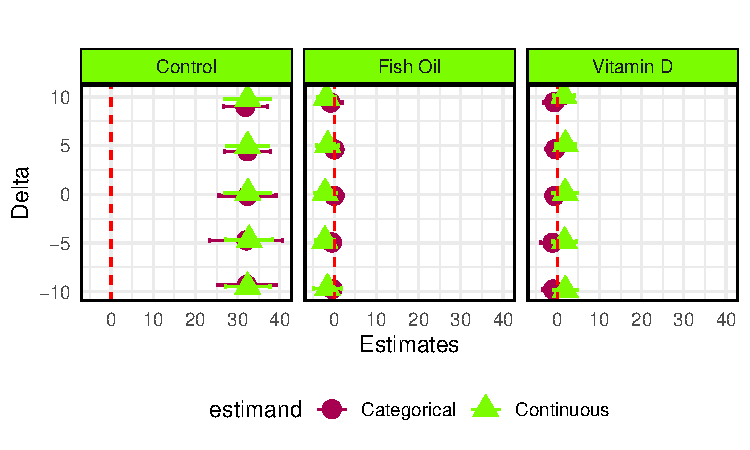
\includegraphics[keepaspectratio]{Final_Report_files/figure-latex/unnamed-chunk-34-1.pdf}}
\caption{Acupuncture data set analysed with different methods; CCA =
complete case analysis; LOCR = last observation carry forward; MO = mean
observation; MI = multiple imputation with linear regression; LME =
linear mixed-effects model without imputation; MI+LME = multiple
imputation followed by linear mixed-effects model.}
\end{figure}

\begin{figure}
\centering
\pandocbounded{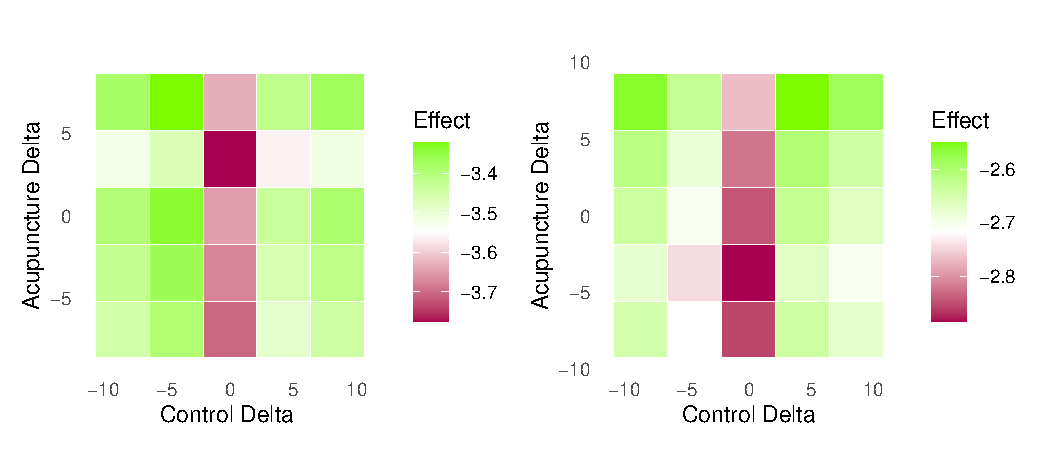
\includegraphics[keepaspectratio]{Final_Report_files/figure-latex/unnamed-chunk-35-1.pdf}}
\caption{VITAL data set analysed with different methods; CCA = complete
case analysis; LOCR = last observation carry forward; MO = mean
observation; MI = multiple imputation with linear regression; LME =
linear mixed-effects model without imputation; MI+LME = multiple
imputation followed by linear mixed-effects model.}
\end{figure}

\subsection{Changing estimand}\label{changing-estimand}

In this section, we explore how changing the estimand (how time is
modeled) to see how that affects our conclusions.

\begin{figure}
\centering
\pandocbounded{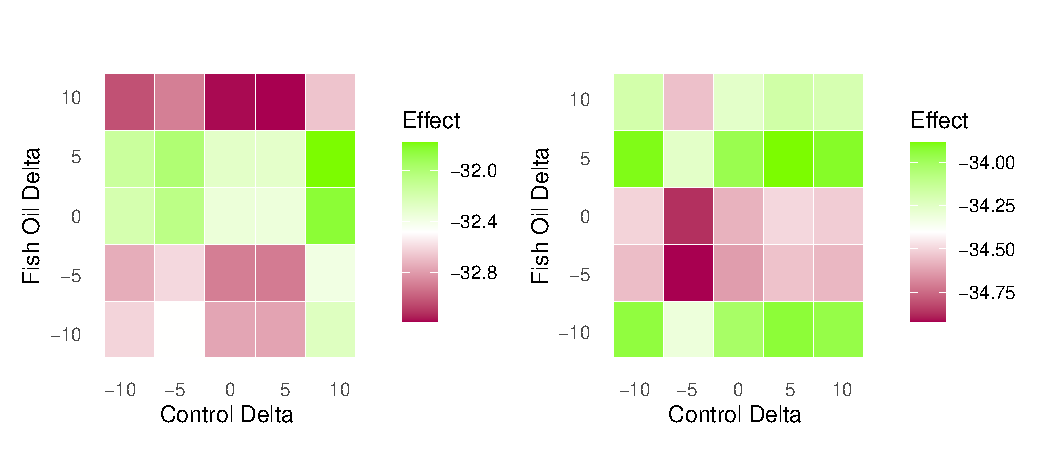
\includegraphics[keepaspectratio]{Final_Report_files/figure-latex/unnamed-chunk-36-1.pdf}}
\caption{Acupuncture data set analysed with different estimands; LME:
linear mix model without imputations; MI+LME: multiple imputation and
linear miex model; Purple line (Original Estimand) estimand: The mean
difference of pain score at the end of study conditional on baseline
pain score, treating time as categorical variable; Green line (Changed
Estimand) estimand: The mean difference of pain score at the end of
study conditional on baseline pain score, treating time as continuous
variable.}
\end{figure}

\begin{figure}
\centering
\pandocbounded{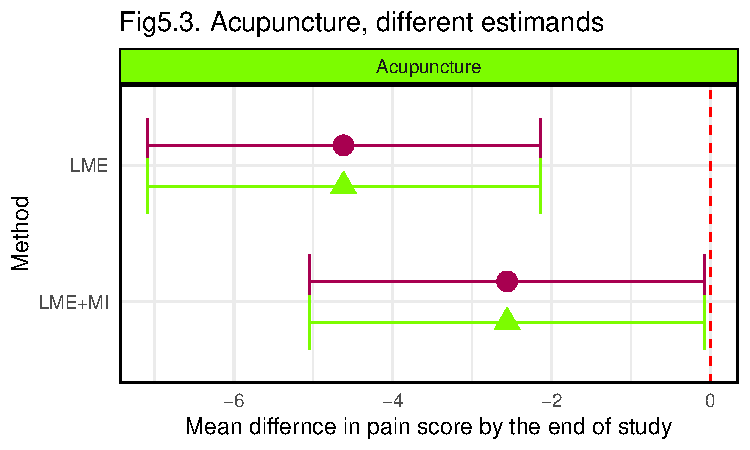
\includegraphics[keepaspectratio]{Final_Report_files/figure-latex/unnamed-chunk-37-1.pdf}}
\caption{VITAL data set analysed with different estimands; LME: linear
mix model without imputations; MI+LME: multiple imputation and linear
miex model; Purple line (Original Estimand) estimand: The mean
difference of pain score at the end of study conditional on baseline
pain score, treating time as categorical variable; Green line (Changed
Estimand) estimand: The mean difference of pain score at the end of
study conditional on baseline pain score, treating time as continuous
variable.}
\end{figure}

\subsection{Changing imputation methods and imputation
numbers}\label{changing-imputation-methods-and-imputation-numbers}

In this session. We keep our estimand treating time as a categorical
variable and using multiple linear regression as substantive model.

We first compared different imputation methods within the FCS framework,
using 5 imputations.

\begin{figure}
\centering
\pandocbounded{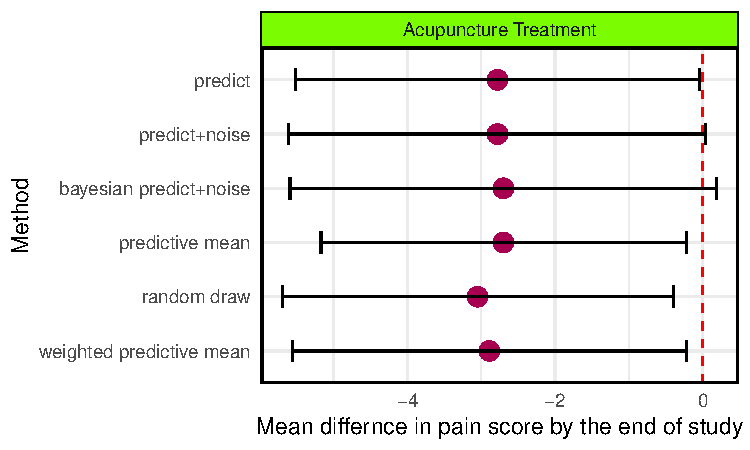
\includegraphics[keepaspectratio]{Final_Report_files/figure-latex/unnamed-chunk-38-1.pdf}}
\caption{Acupuncture data set analysed with different FCS methods}
\end{figure}

\begin{figure}
\centering
\pandocbounded{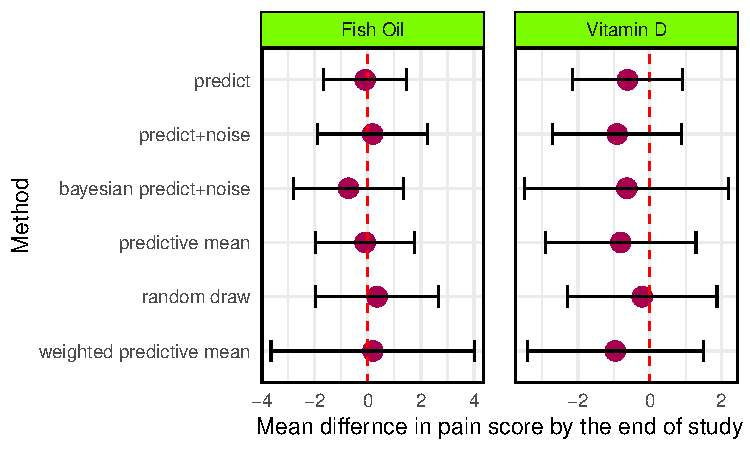
\includegraphics[keepaspectratio]{Final_Report_files/figure-latex/unnamed-chunk-39-1.pdf}}
\caption{VITAL data set analysed with different FCS methods}
\end{figure}

Next, we assess the impact of changing the number of imputations, using
predictive mean method. As introduced in the previous session, we used
\(K=5\), \(K=20\), and \(K=100*\lambda\) (Which is 25 and 50 for
Acupuncture and VITAL data sets accordingly).

\begin{figure}
\centering
\pandocbounded{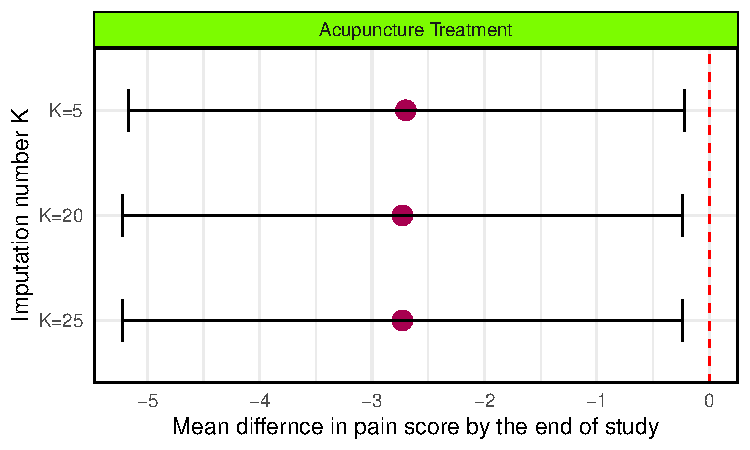
\includegraphics[keepaspectratio]{Final_Report_files/figure-latex/unnamed-chunk-40-1.pdf}}
\caption{Acupuncture data set analysed with different imputation
numbers}
\end{figure}

\begin{figure}
\centering
\pandocbounded{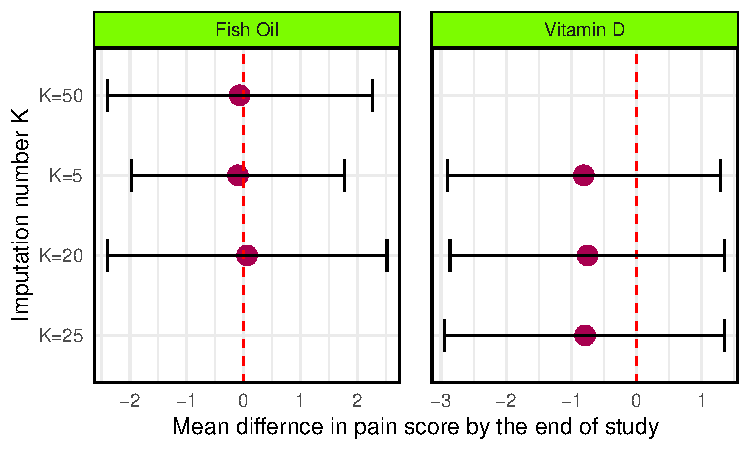
\includegraphics[keepaspectratio]{Final_Report_files/figure-latex/unnamed-chunk-41-1.pdf}}
\caption{VITAL data set analysed with different imputation numbers}
\end{figure}

\subsection{Sensitive analysis}\label{sensitive-analysis-1}

\begin{figure}
\centering
\pandocbounded{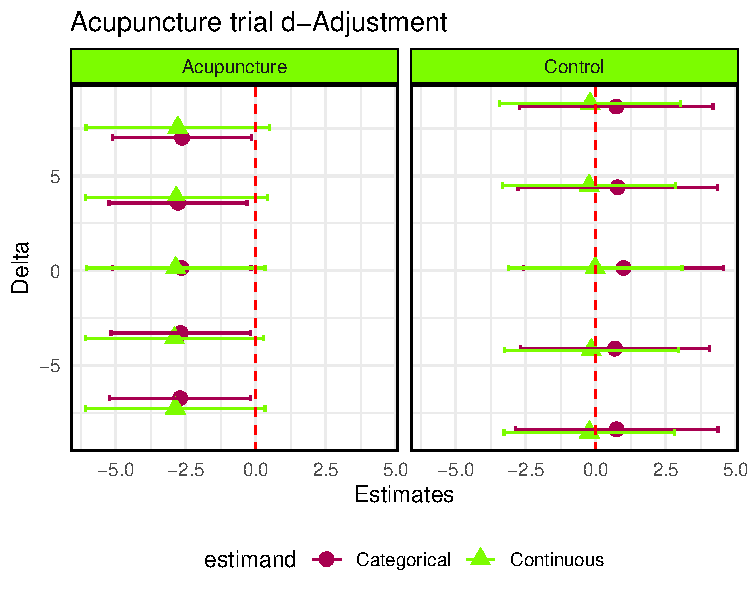
\includegraphics[keepaspectratio]{Final_Report_files/figure-latex/unnamed-chunk-42-1.pdf}}
\caption{Sensitive analysis for Acupuncture data set}
\end{figure}

\begin{figure}
\centering
\pandocbounded{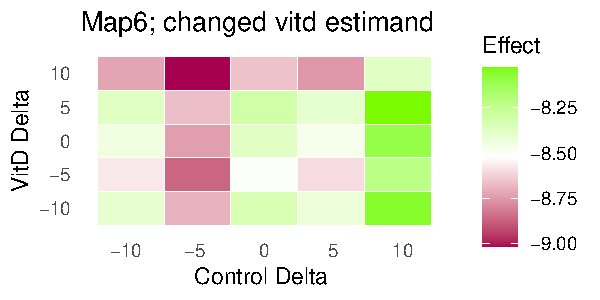
\includegraphics[keepaspectratio]{Final_Report_files/figure-latex/unnamed-chunk-43-1.pdf}}
\caption{Sensitive analysis for VITAL data set}
\end{figure}

The forest plot aims to illustrate the robustness of the estimated
treatment effects under varying missing data assumptions using
\(\delta\) adjustment sensitivity analysis. In figure x which shows the
acupuncture trial results, we can observe the conditional expectation of
headache severity at the final time point of 12 months given the
baseline headache severity and acupuncture treatment under different
\(\delta\) shifts. Similarly we can also observe the conditional
expectation of headache severity at the final time point in the control
group, given baseline headache severity only and no treatment.

Figure Y shows the VITAL results after applying the sensitivity
analysis. In the fish oil panel, we observe the conditional expectation
of knee pain score at 4 years given baseline knee pain score and fish
oil treatment under the different \(\delta\) shifts. The vitamin D panel
shows similar conditional expectation, but the control group shows the
conditional expectation of knee pain score given baseline knee pain
score and no treatment.

The error bars represent the 95\% confidence intervals.

The \(\delta\) parameter shifts the imputed values to simulate scenarios
where the missing data are systematically better or worse than the
observed ones. Positive \(\delta\) values imply better unobserved
outcomes while negative values imply worse. The consistency of estimates
across the \(\delta\) values suggests the treatment effect is robust to
departures from the MAR assumption.

\newpage

\begin{figure}
\centering
\pandocbounded{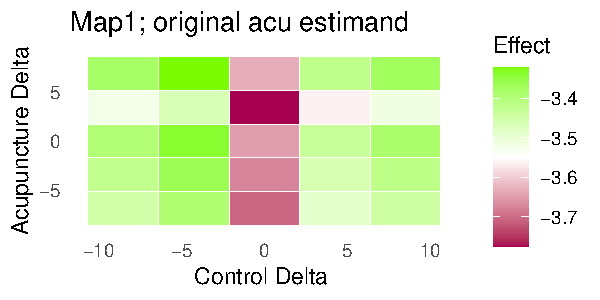
\includegraphics[keepaspectratio]{Final_Report_files/figure-latex/unnamed-chunk-44-1.pdf}}
\caption{original acu estimand}
\end{figure}

\begin{figure}
\centering
\pandocbounded{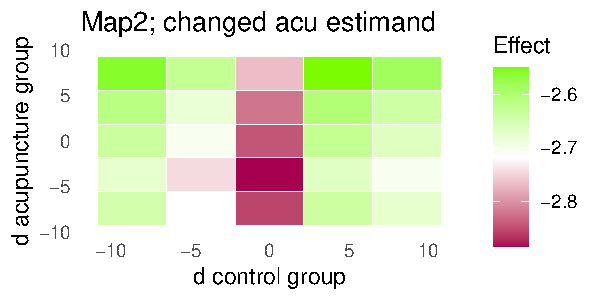
\includegraphics[keepaspectratio]{Final_Report_files/figure-latex/unnamed-chunk-45-1.pdf}}
\caption{changed acu estimand}
\end{figure}

\begin{figure}
\centering
\pandocbounded{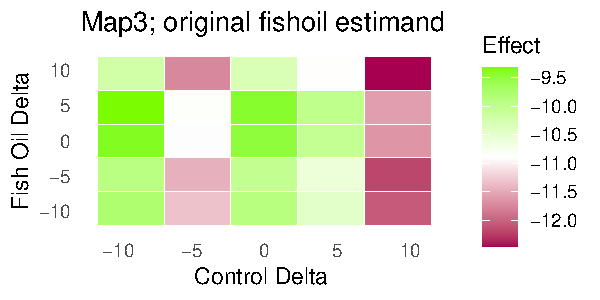
\includegraphics[keepaspectratio]{Final_Report_files/figure-latex/unnamed-chunk-46-1.pdf}}
\caption{original fishoil estimand}
\end{figure}

\begin{figure}
\centering
\pandocbounded{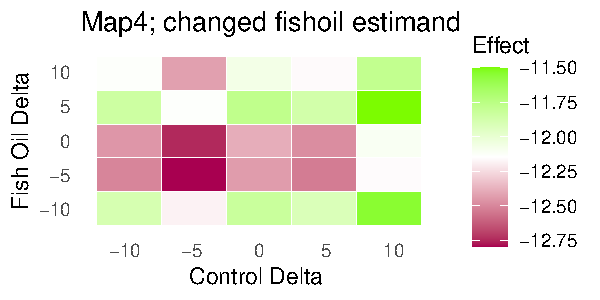
\includegraphics[keepaspectratio]{Final_Report_files/figure-latex/unnamed-chunk-47-1.pdf}}
\caption{changed fishoil estimand}
\end{figure}

\begin{figure}
\centering
\pandocbounded{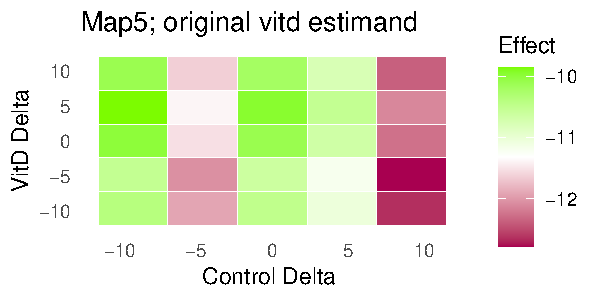
\includegraphics[keepaspectratio]{Final_Report_files/figure-latex/unnamed-chunk-48-1.pdf}}
\caption{original vitd estimand}
\end{figure}

\begin{figure}
\centering
\pandocbounded{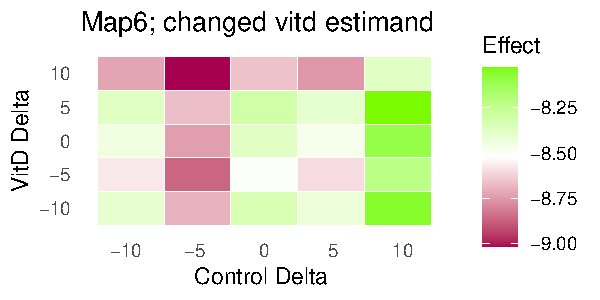
\includegraphics[keepaspectratio]{Final_Report_files/figure-latex/unnamed-chunk-49-1.pdf}}
\caption{changed vitd estimand}
\end{figure}

We created heatmaps plotting the \(\delta\) values for both the control
group and treatment group to visualise the change in treatment effect
when varying the \(\delta\) adjustments under MNAR. The aim here is to
show the robustness of the initial estimated treatment effect when
assumed under a different mechanism. A similar range of colours would be
interpretable as a strong estimate as there was not much change in the
estimate after adding the \(\delta\) shifts.

\section{Discussion}\label{discussion}

Across all analyses, no meaningful difference was observed in the final
treatment effect estimates across the various methods and settings
explored.

However, several points are worth noting:

\begin{itemize}
\item
  In Figures 1 and 2, we observe that methods involving multiple
  imputation (MI) show more variation in the estimated treatment
  effects. This is expected, as MI leverages all available observed
  data, while the other four methods (CAA, LOCF, MO, and LME without
  imputation) use only a subset---typically including only group and
  baseline pain score.
\item
  When we changed the estimand to treat time as a continuous variable,
  the impact was minimal in the Acupuncture study, which is unsurprising
  given that it includes only two follow-up time points. In such cases,
  modeling time continuously offers limited additional information.
\end{itemize}

It is important to emphasize that the goal of this project is not to
revise prior conclusions from the original studies, but rather to gain
practical insights by applying and comparing different methods for
handling missing data.

The fact that our results are broadly consistent across methods should
not be taken to imply that simpler approaches like CCA are equivalent to
more principled methods. Even in a similar future study, the same
results may not hold, especially under different missing data patterns
or assumptions.

This project has highlighted that there are many valid approaches to
handling missing data, and that these can be combined in different ways
depending on the context. It is crucial to understand which methods are
most appropriate under which conditions.

For example:

\begin{itemize}
\item
  LME is a powerful tool for analyzing longitudinal data and can yield
  unbiased results even without imputation---if the assumptions are met.
  However, in the Acupuncture dataset, its utility is limited due to the
  small number of timepoints and its inability to incorporate other
  post-randomisation variables like pain frequency.
\item
  In the VITAL dataset, although there are more timepoints, baseline
  pain scores are sometimes missing. As a result, when fitting LME
  without imputation, individuals with missing baseline values are
  excluded. This exclusion becomes more severe as more covariates with
  missing data are included, potentially leading to substantial loss of
  information. While it is theoretically possible to incorporate
  post-randomisation variables into an LME model by extending the
  covariance structure, this approach is complex and less flexible. In
  contrast, using MI provides a more straightforward way to incorporate
  auxiliary post-randomisation information during the imputation step,
  without requiring modifications to the model structure.
\end{itemize}

\subsection{Limitations of the
project}\label{limitations-of-the-project}

There are several limitations stemming from the inherent characteristics
of the datasets used in this project.These limitations are not a result
of analytic choices but rather reflect the practical boundaries of the
available data.

\begin{itemize}
\item
  \emph{Limited follow-up in Acupuncture dataset:} The Acupuncture study
  includes only two follow-up timepoints (3 and 12 months), which limits
  the ability to model time flexibly or detect subtle longitudinal
  trends. As a result, methods like linear mixed-effects models offer
  limited additional benefit in this context.
\item
  \emph{Weak treatment effect in VITAL:} The VITAL dataset shows
  relatively small therapeutic effects, making it difficult to detect
  meaningful differences between methods. This also reduces the
  practical impact of using more advanced imputation strategies.
\item
  \emph{No known data-generating mechanism:} Since we are working with
  one-off samples from an unknown data-generating process and a true,
  unobserved treatment effect---rather than simulated data---we cannot
  evaluate the performance of different analytical methods against a
  known ground truth. This limits our ability to draw general
  conclusions about their long-run properties.
\end{itemize}

\subsection{Future work}\label{future-work}

In addition, there are methodological aspects that could be improved or
explored further in future work. These include choices related to model
specification, variable adjustment, and the diversity of imputation
techniques employed. Addressing these areas could enhance the robustness
and generalizability of findings, especially in more complex or
data-rich clinical contexts.

\begin{itemize}
\item
  \emph{Model specification:} Both linear regression and LME rely on
  assumptions such as linearity and normally distributed residuals.
  While these assumptions were not formally tested, the sample size in
  the VITAL dataset is likely large enough for the central limit theorem
  to provide valid inference. That said, future work could benefit from
  visual checks of residuals and distributions of pain scores at each
  timepoint to give a clearer sense of model fit and outcome behaviour.
\item
  \emph{Imputation strategy:} In the most of our analysis, we used
  predictive mean matching for imputing missing variables. While this is
  a valid and robust approach, many other imputation models as we
  introduced were not explored in detail. These could be considered in
  future work to assess sensitivity to imputation method.
\item
  \emph{Covariate adjustment in substantive models:} Our analysis models
  adjusted only for treatment group and baseline pain score in our
  substantive model to ensure comparability across methods. This
  low-level of adjustment in the substantive model is the reason we
  observed larger discrepancies between results using MI and those not
  using MI, as a fuller set of covariates was used during MI. Future
  work could explore how more complex substantive model specifications
  interacts with MI and influences treatment effect estimates.
\end{itemize}

\phantomsection\label{refs}
\begin{CSLReferences}{1}{0}
\bibitem[\citeproctext]{ref-bodner_bodner2008what_2008}
Bodner, Todd E. 2008. {``(Bodner2008)what Improves with Increased
Missing Data Imputations?''} \emph{Structural Equation Modeling: A
Multidisciplinary Journal} 15 (4): 651--75.
\url{https://doi.org/10.1080/10705510802339072}.

\bibitem[\citeproctext]{ref-carpenter_multiple_2023}
Carpenter, James R., Jonathan W. Bartlett, Tim P. Morris, Angela M.
Wood, Matteo Quartagno, and Michael G. Kenward. 2023. \emph{Multiple
Imputation and Its Application}. 2nd ed. Statistics in Practice. Wiley.
\url{https://onlinelibrary.wiley.com/doi/book/10.1002/9781119756118}.

\bibitem[\citeproctext]{ref-graham_how_2007}
Graham, John W., Allison E. Olchowski, and Tamika D. Gilreath. 2007.
{``How Many Imputations Are Really Needed? Some Practical Clarifications
of Multiple Imputation Theory.''} \emph{Prevention Science: The Official
Journal of the Society for Prevention Research} 8 (3): 206--13.
\url{https://doi.org/10.1007/s11121-007-0070-9}.

\bibitem[\citeproctext]{ref-royston_royston2004multiple_2004}
Royston, Patrick. 2004. {``(Royston2004)multiple Imputation of Missing
Values.''} \emph{The Stata Journal} 4 (3): 227--41.
\url{https://doi.org/10.1177/1536867X0400400301}.

\bibitem[\citeproctext]{ref-noauthor_rubin1987_1987}
\emph{(Rubin1987) Multiple Imputation for Nonresponse in Surveys}. 1987.
John Wiley \& Sons, Ltd.
\url{https://doi.org/10.1002/9780470316696.fmatter}.

\bibitem[\citeproctext]{ref-white_multiple_2011-1}
White, Ian R., Patrick Royston, and Angela M. Wood. 2011. {``Multiple
Imputation Using Chained Equations: Issues and Guidance for Practice.''}
\emph{Statistics in Medicine} 30 (4): 377--99.
\url{https://doi.org/10.1002/sim.4067}.

\end{CSLReferences}

\bibliographystyle{unsrt}
\bibliography{Missing\_data\_references.bib}


\end{document}
